% ==============================================================================
% MAIN.TEX - ENTRY POINT UNTUK TEMPLATE BUKU / MODUL
% ==============================================================================

\documentclass[12pt, a4paper]{book}

% --- Import Preamble ---
% ==============================================================================
% PREAMBLE: TEMPLATE MODUL / BUKU STANDAR
% ==============================================================================

\usepackage[utf8]{inputenc}
\usepackage[T1]{fontenc}
\usepackage[indonesian]{babel} % Support for Bahasa Indonesia
\usepackage{geometry}
\usepackage{graphicx}
\usepackage{xcolor}
\usepackage{fancyhdr}
\usepackage{titlesec}
\usepackage{tocloft}
\usepackage{booktabs}
\usepackage{tabularx}
\usepackage{array}
\newcolumntype{L}{>{\raggedright\arraybackslash}X}
\newcolumntype{C}{>{\centering\arraybackslash}X}
\newcolumntype{R}{>{\raggedleft\arraybackslash}X}
\usepackage{caption}
\usepackage{subcaption}
\usepackage{hyperref}
\usepackage{tikz}
\usepackage{setspace}
\usepackage{enumitem}
\usepackage{mathptmx} % Use Times New Roman style font

% --- Global Style Adjustments ---
\onehalfspacing % Set line spacing to 1.5
\setlist[enumerate]{leftmargin=1.5cm, labelsep=0.5cm} % Standardize list margins
\setlist[itemize]{leftmargin=1.5cm, labelsep=0.5cm}
\setlength{\parindent}{1cm} % Standard paragraph indentation
\setlength{\parskip}{0pt}   % No extra space between paragraphs
\sloppy                      % Prevent overfull hbox in justified text

% --- Geometri Halaman ---
\geometry{
    a4paper,
    top=1.18in,
    bottom=1.58in,
    left=1.18in,
    right=1.18in,
    headheight=15pt, % Recommended by fancyhdr
    headsep=0.47in,  % 1.18in - 15pt - 0.5in = 0.47in approx
    footskip=1.08in  % 1.58in - 0.5in = 1.08in
}

% --- Header & Footer ---
\fancypagestyle{plain}{ % Re-define plain style for chapter start pages
    \fancyhf{}
    \fancyhead[C]{
        \begin{tikzpicture}[remember picture,overlay]
            \node[anchor=north west, fill=gray!20, minimum width=\paperwidth-1cm, minimum height=1.8cm, xshift=1cm] at (current page.north west) {};
            \node[anchor=east] at ([xshift=-1.18in, yshift=-1.0cm]current page.north east) {
                
\includegraphics[height=1.2cm]{image/Logo_Universitas_Telkom_Horizontal.png}
            };
        \end{tikzpicture}
    }
    \fancyfoot[R]{\thepage}
    \renewcommand{\headrulewidth}{0pt}
}

\pagestyle{fancy}
\fancyhf{}
\fancyhead[C]{
    \begin{tikzpicture}[remember picture,overlay]
        \node[anchor=north west, fill=gray!20, minimum width=\paperwidth-1cm, minimum height=1.8cm, xshift=1cm] at (current page.north west) {};
        \node[anchor=east] at ([xshift=-1.18in, yshift=-1.0cm]current page.north east) {
            
\includegraphics[height=1.2cm]{image/Logo_Universitas_Telkom_Horizontal.png}
        };
    \end{tikzpicture}
}
\fancyfoot[R]{\thepage}
\renewcommand{\headrulewidth}{0pt}
\renewcommand{\footrulewidth}{0pt}

% --- Styling Bab & Seksi ---
\titleformat{\chapter}[display]
  {\normalfont\bfseries\centering}
  {\Large\chapterservicename\ \Roman{chapter}}
  {1ex}
  {\huge\MakeUppercase}
\titlespacing*{\chapter}{0pt}{-20pt}{40pt}

\titleformat{\section}
  {\normalfont\Large\bfseries\color{black}}
  {\thesection}{1em}{}

\titleformat{\subsection}
  {\normalfont\large\bfseries\color{black}}
  {\thesubsection}{1em}{}

\titleformat{\subsubsection}
  {\normalfont\normalsize\bfseries\color{black}}
  {\thesubsubsection}{1em}{}

% --- Section Numbering Adjustments ---
\setcounter{secnumdepth}{3} % Allow numbering for subsubsections
\setcounter{tocdepth}{3}    % Include subsubsections in TOC
\renewcommand{\thesection}{\arabic{chapter}.\arabic{section}} % 1.1
\renewcommand{\thesubsection}{\thesection.\arabic{subsection}} % 1.1.1
\renewcommand{\thesubsubsection}{\thesubsection.\arabic{subsubsection}} % 1.1.1.1

% --- Hyperref Setup ---
\hypersetup{
    colorlinks=true,
    linkcolor=black,
    filecolor=magenta,      
    urlcolor=black,
    citecolor=blue,
    pdftitle={Book FAR - Template Modul},
}

% --- Custom Commands ---
\newcommand{\chapterservicename}{BAB} % Standard for Indonesian "BAB"

% --- Definisi Daftar Lampiran ---
\newcommand{\listappendixname}{Daftar Lampiran}
\newlistof{lampiran}{lop}{\listappendixname}
\renewcommand{\cftloptitlefont}{\huge\bfseries}
\renewcommand{\cftafterloptitle}{}
\setlength{\cftbeforeloptitleskip}{0pt}
\setlength{\cftafterloptitleskip}{0.5cm}

% Biar Daftar Lampiran muncul di TOC
\newcommand{\addlampiran}[1]{%
  \refstepcounter{lampiran}%
  \addcontentsline{lop}{lampiran}{\protect\numberline{Lampiran \thelampiran}#1}%
}

% Prevent hyphenation for Indonesian
\hyphenpenalty=10000
\exhyphenpenalty=10000


\begin{document}

% --- Front Matter (Judul, TOC, dsb) ---
\frontmatter
% ==============================================================================
% FRONTMATTER: TITLE PAGE & TOC
% ==============================================================================

\begin{titlepage}
    \centering
    % \vspace*{2cm}
    
    {\Large\bfseries\color{black} Food AI Rescue : Platform Pengolahan dan Pendistribusian Makanan Sisa Berbasis AI\par}
    % \vspace{0.2cm}
    {\Large\bfseries\color{black} Food AI Rescue: An AI-Based Platform for the Processing and Distribution of Food Waste\par}
    % \vspace{0.5cm}
    {\bfseries Dokumen ini ditujukan untuk memenuhi persyaratan Mata Kuliah Tugas Akhir\par}
    
    % \vspace{1cm}
    
    % Placeholder for logo
    \vspace{1cm}
    
\includegraphics[width=0.5\textwidth]{image/logo.png} \par
    
    \vfill
    {\large Disusun Oleh, \\}
    {\large 607012400075 - Shafnat Fuaini Ramadhan, \\}
    {\Large PROGRAM STUDI D3 SISTEM INFORMASI \\}
    {\Large FAKULTAS ILMU TERAPAN \\}
    {\Large UNIVERSITAS TELKOM \\}
    {\Large BANDUNG \\}
    {\large 2026}
\end{titlepage}

% --- LEMBAR PERSEMBAHAN ---
\newpage
\thispagestyle{empty}
% \vspace*{4cm}
\begin{center}
    \Large\bfseries LEMBAR PERSEMBAHAN
\end{center}

% \vspace{1.5cm}

\begin{center}
    \itshape
    \large
    Laporan Tugas Akhir ini penulis persembahkan dengan penuh rasa syukur dan cinta kepada: \\
    
    \vspace{1cm}
    \textbf{Orang Tua Tercinta,} \\
    Mama dan Bapak, atas doa-doa tulus di setiap sujudnya, \\
    kasih sayang yang tiada batas, serta dukungan yang luar biasa hingga penulis sampai di titik ini. \\
    
    \vspace{1cm}
    \textbf{Keluarga Besar,} \\
    Terima kasih telah menjadi pendukung setia dan selalu memberikan semangat di kala lelah. \\
    
    \vspace{1cm}
    \textbf{Seluruh Pihak,} \\
    Yang telah membantu, membimbing, dan memberikan inspirasi dalam penyusunan karya ini, \\
    baik secara langsung maupun tidak langsung. \\
    
    \vspace{1.5cm}
    \textit{“Sesungguhnya sesudah kesulitan itu ada kemudahan.”} \\
    (QS. Al-Insyirah: 6)
\end{center}

% --- LEMBAR PENGESAHAN ---
\newpage
\addcontentsline{toc}{section}{LEMBAR PENGESAHAN}

\vspace{1.5cm}
\begin{center}
    {\large\bfseries LEMBAR PENGESAHAN \par}
    
    \vspace{2cm}
    
    {\large\bfseries FOOD AI RESCUE: PLATFORM PENGOLAHAN DAN PENDISTRIBUSIAN MAKANAN SISA BERBASIS AI \par}
    \vspace{0.3cm}
    {\large\itshape\bfseries FOOD AI RESCUE: AN AI-BASED PLATFORM FOR THE PROCESSING AND DISTRIBUTION OF FOOD WASTE \par}
\end{center}

\vspace{2cm}

\noindent
\begin{tabularx}{\textwidth}{@{} L r @{}}
    Penulis & \\
    \bfseries Shafnat Fuaini Ramadhan \\ NIM 607012400075 & 
    \begin{tabular}[t]{c} \\[0cm] 
        
\includegraphics[height=1.5cm]{image/signature.png} \\ % Placeholder for signature
        \rule{6.5cm}{0.4pt} 
    \end{tabular} \\
\end{tabularx}

\vspace{1.5cm}

\noindent
\begin{tabularx}{\textwidth}{@{} L r @{}}
    Dosen Pembimbing 1 & \\
    \bfseries Robbi Hendriyanto, S.T., M.T \\ NIP 13850086 & \begin{tabular}[t]{c} \\[0cm] \rule{6.5cm}{0.4pt} \end{tabular} \\ 
\end{tabularx}

\vfill

\noindent
Tanggal Pengesahan: 4 April 2026

% --- KATA PENGANTAR ---
\newpage
\begin{center}
    {\large\bfseries KATA PENGANTAR \par}
\end{center}
\addcontentsline{toc}{section}{KATA PENGANTAR}
\vspace{0.5cm}

Puji syukur penulis panjatkan ke hadirat Allah Subhanahu Wa Ta'ala karena atas rahmat dan karunia-Nya, penulis dapat menyelesaikan Tugas Akhir ini dengan baik. Tugas Akhir ini disusun sebagai salah satu syarat akademik yang harus dipenuhi dalam menyelesaikan studi.

Proses penyusunan Tugas Akhir ini bukan hanya perjalanan akademik, tetapi juga perjalanan kesabaran dan keteguhan. Ada malam-malam yang panjang, ada langkah-langkah yang sempat ragu, namun selalu ada doa dan dukungan yang menguatkan. Dengan penuh ketulusan, penulis menyampaikan terima kasih yang sebesar-besarnya kepada:

\begin{enumerate}
    \item Keluarga tercinta, terutama kepada Mama, Bapak, Kakak, dan kedua adik penulis, yang selalu memberikan doa, kasih sayang, serta kekuatan untuk terus melangkah.
    \item Bapak Robbi Hendriyanto, S.T., M.T., selaku dosen pembimbing yang telah memberikan bimbingan, masukan, dan arahan selama proses penyusunan Tugas Akhir ini.
    \item Bapak Dr. Hanung Nindito Prasetyo, S.Si., M.T. dan Bapak Hanang Priambodo, S.T., M.Kom selaku dosen penguji yang telah memberikan masukan, kritik, dan saran yang membangun demi perbaikan Tugas Akhir ini.
    \item Sahabat-sahabat seperjuangan yang namanya tidak dapat disebutkan satu per satu, yang telah berbagi semangat, lelah, dan kebersamaan hingga tiba pada tahap ini.
    \item Semua pihak yang dengan caranya masing-masing memberi warna dalam perjalanan akademik penulis.
    \item Dan untuk diri sendiri, terima kasih karena telah bertahan saat menyerah tampak lebih mudah, terima kasih karena tetap berjalan meski langkah terasa berat, dan terima kasih karena terus percaya bahwa setiap langkah kecil pada akhirnya akan membawa sampai di sini.
\end{enumerate}

\vspace{1cm}
\noindent
Penulis menyadari bahwa masih terdapat berbagai keterbatasan dalam penelitian ini. Oleh karena itu, kritik dan saran yang membangun sangat diharapkan untuk pengembangan lebih lanjut. Semoga Tugas Akhir ini dapat memberikan manfaat bagi dunia pendidikan, industri kuliner, serta masyarakat luas.

\vspace{1cm}
\begin{flushright}
    \begin{singlespace}
        Bandung, April 2026 \\
        \vspace{1cm}
        \begin{tabular}{c}
            
\includegraphics[height=1.5cm]{image/signature.png} \\ 
            \rule{4cm}{0.4pt} \\
            \bfseries Penulis
        \end{tabular}
    \end{singlespace}
\end{flushright}

% --- PERNYATAAN ---
\newpage
\begin{center}
    {\large\bfseries PERNYATAAN \par}
\end{center}
\addcontentsline{toc}{section}{PERNYATAAN}
\vspace{0.5cm}
Dengan ini saya menyatakan bahwa: 
\begin{enumerate}
    \item karya tulis ini adalah asli dan belum pernah diajukan untuk mendapatkan gelar 
    akademik (Ahli Madya, Sarjana, Magister dan Doktor), baik di Fakultas Ilmu 
    Terapan Universitas Telkom maupun di perguruan tinggi lainnya;
    \item karya tulis ini merupakan bagian dari Tugas Akhir yang dikerjakan secara 
    individu.
    \item karya tulis ini murni gagasan, rumusan, dan penelitian saya sendiri, tanpa 
    bantuan pihak lain, kecuali arahan tim pembimbing atau tim promotor atau 
    penguji; 
    \item dalam karya tulis ini tidak terdapat cuplikan karya atau pendapat yang telah 
    ditulis atau dipublikasikan orang lain, kecuali secara tertulis dengan jelas 
    dicantumkan sebagai acuan dalam naskah dengan menyebutkan nama 
    pengarang dan dicantumkan dalam daftar pustaka;
    \item saya mengijinkan karya tulis ini dipublikasikan oleh Fakultas Ilmu Terapan 
    Universitas Telkom, dengan tetap mencantumkan saya sebagai penulis; dan
\end{enumerate}

\vspace{0.3cm}
\noindent
Pernyataan ini saya buat dengan sesungguhnya dan apabila pada kemudian hari 
terdapat penyimpangan dan ketidakbenaran dalam pernyataan ini maka saya 
bersedia menerima sanksi akademik berupa pencabutan gelar yang telah 
diperoleh karena karya tulis ini, serta sanksi lainnya sesuai norma yang berlaku 
di Fakultas Ilmu Terapan Universitas Telkom. 

\vspace{1cm}
\begin{flushleft}
    \begin{singlespace}
        Bandung, April 2026 \\
        \vspace{1cm}
        \begin{tabular}{c}
            
\includegraphics[height=1.5cm]{image/signature.png} \\ 
            \rule{4cm}{0.4pt} \\
            Shafnat Fuaini Ramadhan
        \end{tabular}
    \end{singlespace}
\end{flushleft}

% --- PERNYATAAN ---
% \newpage
% \section*{PERNYATAAN ORISINALITAS}
% \addcontentsline{toc}{section}{PERNYATAAN ORISINALITAS}
% \vspace{1cm}
% Saya yang bertandatangan di bawah ini:
% \vspace{1cm}
% \begin{tabular}{p{3cm} p{1cm} p{10cm}}
%     Nama & : & Shafnat Fuaini Ramadhan \\
%     NIM & : & 607012400075 \\
%     Judul & : & Food AI Rescue \\
% \end{tabular}
% \vspace{1.5cm}
% Menyatakan dengan sebenarnya bahwa Tugas Akhir ini adalah hasil karya saya sendiri, dan semua sumber baik yang dikutip maupun dirujuk telah saya nyatakan dengan benar.
% \vspace{2cm}
% \begin{flushright}
%     Bandung, \today \\
%     \vspace{2cm}
%     \textbf{Shafnat Fuaini Ramadhan}
% \end{flushright}

% --- ABSTRAK (INDONESIA) ---
\newpage
\begin{center}
    {\Large\bfseries ABSTRAK \par}
    \addcontentsline{toc}{section}{ABSTRAK}
    \vspace{0.5cm}
    {\large\bfseries Food AI Rescue \par}
    \vspace{0.5cm}
    Oleh: \\
    Shafnat Fuaini Ramadhan \\
    607012400075 \\
\end{center}
\vspace{1cm}
Food AI Rescue adalah sebuah sistem yang... [Tuliskan abstrak Anda di sini dalam bahasa Indonesia. Abstrak merupakan ringkasan singkat dari tugas akhir Anda meliputi masalah, tujuan, metode, dan hasil.]
\vspace{1cm}
\noindent \textbf{Kata Kunci:} AI, Food Rescue, Sistem Informasi, Telkom University.

% --- ABSTRACT (ENGLISH) ---
\newpage
\begin{center}
    {\Large\bfseries ABSTRACT \par}
    \addcontentsline{toc}{section}{ABSTRACT}
    \vspace{0.5cm}
    {\large\bfseries\itshape Food AI Rescue \par}
    \vspace{0.5cm}
    By: \\
    Shafnat Fuaini Ramadhan \\
    607012400075 \\
\end{center}
\vspace{1cm}
\textit{Food AI Rescue is a system that... [Write your abstract here in English. The abstract is a concise summary of your final project including the problem, objectives, methods, and results.]}
\vspace{1cm}
\noindent \textbf{Keywords:} \textit{AI, Food Rescue, Information System, Telkom University.}

\newpage
\tableofcontents
\newpage
\listoffigures
\newpage
\listoftables
\newpage


% --- Main Matter (Bab-bab utama) ---
\mainmatter

% Gunakan \include atau \input untuk memanggil file bab dari folder 'bab'
% ==============================================================================
% BAB 1: PENDAHULUAN
% ==============================================================================

\chapter{Pendahuluan}
\label{chapter:pendahuluan}
\section{Latar Belakang}
Indonesia menghadapi tantangan paradoks ketahanan pangan yang sangat serius. Di satu sisi, Indonesia tercatat menghasilkan timbulan Food Loss and Waste (FLW) yang sangat masif, yakni diperkirakan mencapai 23 hingga 48 juta ton (atau sekitar 115 hingga 184 kilogram per kapita) setiap tahunnya (Bappenas, 2021). Angka ini menjadikan Indonesia sebagai salah satu negara penghasil limbah makanan terbesar di dunia (Waluyo \& Kharisma, 2023). Ironisnya, di tengah tingginya angka pemborosan ini, Indonesia masih berhadapan dengan masalah kerawanan pangan dan malnutrisi, termasuk tingginya prevalensi balita stunting yang mencapai 21,6\% pada tahun 2022 (Lybaws et al., 2025). Padahal, secara kumulatif, jumlah makanan yang hilang dan terbuang tersebut memiliki kandungan nutrisi energi yang cukup untuk memberi makan 61 hingga 125 juta orang, atau setara dengan 29\% hingga 47\% dari total populasi Indonesia (Bappenas, 2021).\\
\\
Timbulan limbah makanan ini tidak hanya memperburuk kondisi sosial, tetapi juga memberikan dampak yang merugikan secara ekonomi dan ekologis. Secara ekonomi, FLW di Indonesia menyebabkan kerugian yang diperkirakan mencapai Rp 213 triliun hingga Rp 551 triliun per tahun, angka yang setara dengan 4\% hingga 5\% dari total Produk Domestik Bruto (PDB) nasional (Bappenas, 2021; Taufiqi et al., 2025),. Dari perspektif lingkungan, sisa makanan secara konsisten mendominasi komposisi sampah nasional, yakni mencapai lebih dari 40\% dari total timbulan sampah (Waluyo \& Kharisma, 2023). Akumulasi sampah organik yang membusuk ini menyumbang emisi Gas Rumah Kaca (GRK) sebesar 1.702,9 Mt CO2-eq selama kurun waktu 20 tahun, yang merepresentasikan 7,29\% dari total emisi GRK Indonesia (Bappenas, 2021).\\
\\
Titik kritis penyumbang limbah makanan terbesar di Indonesia berada pada tahap konsumsi, baik yang bersumber dari rumah tangga maupun dari sektor Hospitality, Restaurant, dan Cafe atau HORECA (Bappenas, 2021). Praktik pemborosan di sektor penyedia makanan sering kali dipicu oleh ketiadaan sistem distribusi dan regulasi manajemen sisa makanan yang memadai (Bappenas, 2021). Sebenarnya, terdapat keinginan dari berbagai pihak HORECA untuk menyalurkan makanan surplus mereka kepada pihak yang membutuhkan, namun niat ini terhambat oleh berbagai kekhawatiran operasional (Bappenas, 2021). Pelaku usaha khawatir makanan donasi tersebut disalahgunakan atau diperjualbelikan kembali oleh oknum tidak bertanggung jawab (Bappenas, 2021). Lebih jauh lagi, ketiadaan standar penanganan memunculkan ketakutan dan penghindaran liabilitas akan ancaman tuntutan hukum apabila terjadi kasus keracunan makanan akibat penurunan kualitas pangan saat didistribusikan (Bappenas, 2021; Bachtiar et al., 2024),.\\
\\
Untuk memecahkan kebuntuan "keterhubungan yang terputus" antara penyedia surplus pangan dan masyarakat rentan, serta sejalan dengan komitmen Indonesia terhadap pencapaian Sustainable Development Goals (SDGs) target 12.3 tentang pengurangan food waste (Bappenas, 2021; Taufiqi et al., 2025),, diperlukan sebuah intervensi teknologi agregator digital. Oleh karena itu, penelitian ini mengusulkan pengembangan platform Food AI Rescue (FAR). Sistem ini hadir untuk menyediakan fasilitas pencocokan logistik donasi pangan secara real-time yang dilengkapi dengan fitur verifikasi kelayakan visual makanan menggunakan kecerdasan buatan (Computer Vision). Melalui sistem penjamin mutu dan transparansi pelaporan ini, keraguan pelaku usaha untuk menyalurkan makanan dapat diatasi, sehingga beban limbah makanan dapat diubah menjadi nilai kemanfaatan sosial yang inklusif dan terukur.\\

% Rumusan Masalah
\section{Rumusan Masalah}
Berdasarkan latar belakang sebagaimana diuraikan di atas, maka dapat diidentifikasi permasalahan sebagai berikut:
\begin{enumerate}
    \item Bagaimana merancang sebuah platform agregator digital (Food AI Rescue) yang mampu memecahkan masalah "keterhubungan yang terputus" dengan mengintegrasikan logistik donasi pangan antara penyedia (HORECA) dan masyarakat rentan secara real-time?
    \item Bagaimana mengimplementasikan teknologi kecerdasan buatan (Computer Vision) pada platform untuk memverifikasi kelayakan visual makanan secara otomatis, guna memitigasi kekhawatiran liabilitas (tuntutan hukum/keracunan) dari para pelaku usaha?
    \item Bagaimana membangun sistem manajemen pelaporan yang transparan dan terukur untuk memastikan makanan donasi tepat sasaran dan mencegah terjadinya praktik penyalahgunaan oleh oknum yang tidak bertanggung jawab?
\end{enumerate}

% Tujuan
\section{Tujuan}
Berdasarkan identifikasi masalah diatas, maka dapat dirumuskan tujuan dari penulisan proyek akhir ini adalah sebagai berikut:
\begin{enumerate}
    \item Merancang dan membangun platform agregator logistik digital (Food AI Rescue) berbasis Progressive Web App (PWA yang berfungsi sebagai jembatan distribusi real-time (menggunakan algoritma AI Matching \& Allocation) untuk memecahkan masalah "keterhubungan yang terputus" antara penyedia surplus pangan halal dan komunitas rentan.
    \item Mengimplementasikan teknologi kecerdasan buatan (Computer Vision) melalui fitur AI Quality Verification guna menganalisis dan memvalidasi kelayakan visual serta kebersihan foto makanan sebelum didistribusikan, sehingga mampu memberikan jaminan mutu dan menekan kekhawatiran liabilitas atau risiko keracunan dari pihak pelaku usaha.
    \item Membangun dasbor sistem pelaporan dan analitik dampak (AI Impact Analytics) yang transparan dan terukur untuk memantau rekam jejak donasi secara digital (traceability), mencegah praktik penyalahgunaan distribusi (double-claim), serta menyajikan data keberhasilan seperti estimasi pengurangan jejak karbon (CO$_2$) dan nilai SROI (Social Return on Investment) bagi para mitra donatur.
\end{enumerate}

% Cangkupan pengerjaan
\section{Cakupan Pengerjaan}
Cakupan pengerjaan Tugas Akhir ini sebagai berikut:
\begin{enumerate}
    \item Ruang Lingkup Aplikasi: Sistem yang dibangun adalah aplikasi berbasis web (Progressive Web App/PWA) yang berfungsi khusus sebagai agregator logistik untuk memfasilitasi donasi makanan surplus halal yang masih layak konsumsi secara gratis atau non-komersial
    \item Batasan Pengguna (Aktor): Sistem membatasi interaksi pada lima peran pengguna, yaitu: Mitra Penyedia/Donatur (mengunggah stok), Mitra Penerima (mencari dan mengklaim makanan), Relawan (armada logistik sosial pengantar makanan), Admin Pengelola (memverifikasi pengguna dan memantau dampak), serta Super Admin (pemeliharaan teknis)
    \item Batasan Fitur dan Teknologi Utama: Pengembangan sistem dibatasi pada tiga modul kecerdasan buatan utama:
    \begin{enumerate}
        \item AI Matching \& Allocation: Pencocokan stok makanan dengan penerima terdekat menggunakan pelacakan radius GPS.
        \item AI Quality \& Halal Verification: Integrasi dengan Application Programming Interface (API) Gemini 3 Engine untuk memindai foto makanan (menggunakan kamera perangkat) guna memberikan prediksi kelayakan visual, kebersihan, dan estimasi kehalalan.
        \item AI Impact Analytics: Dasbor pelaporan yang mencatat riwayat transaksi untuk mengkalkulasi dampak sosial (Social Return on Investment/SROI) dan estimasi reduksi jejak karbon (CO$_2$).
    \end{enumerate}
    \item Batasan Lingkup Geografis dan Operasional: Pengujian dan implementasi sistem (pilot project) dibatasi di wilayah Desa Lengkong, Kecamatan Bojongsoang, Kabupaten Bandung. Sistem juga tidak menyediakan armada logistik komersial sendiri, melainkan hanya memfasilitasi koordinasi penjemputan (diambil langsung oleh penerima atau diantarkan oleh Relawan lokal).
    \item Batasan Teknis dan Keamanan AI: Aplikasi dirancang dengan teknologi Front-End React JS dan Back-End Node/PHP (REST API) menggunakan database MySQL. Aplikasi mewajibkan adanya koneksi internet aktif, akses lokasi (GPS), dan izin kamera keras. Analisis kualitas makanan oleh AI (Food Guard AI) hanya bertindak sebagai bantuan verifikasi visual awal, sedangkan validasi akhir keamanan pangan tetap menjadi tanggung jawab manusia (Admin atau Mitra Penerima) sebelum makanan dikonsumsi.
\end{enumerate}

% Tahapan pengerjaan
\section{Tahapan Pengerjaan}
Pengembangan platform Food AI Rescue (FAR) mengadopsi pendekatan pengerjaan yang iteratif, kolaboratif, dan berbasis Minimum Viable Product (MVP). Pelaksanaan program ini dirancang berlangsung selama kurang lebih (waktu pengerjaan) minggu dengan tahapan terstruktur yang berfokus pada adopsi teknologi oleh masyarakat sasaran. Berikut adalah tahapan pengerjaan yang dilakukan:
\begin{enumerate}
    \item Fase Inisiasi, Sosialisasi, dan Perancangan Sistem (Minggu 1 - 2)
    \begin{itemize}
        \item Sosialisasi dan Koordinasi: Tim melakukan observasi dan koordinasi langsung dengan pengurus Komunitas Halal Bandung (KHB) di Desa Lengkong untuk merumuskan alur program. Pada fase ini juga dilakukan rekrutmen dan pembentukan "Tim Lokal" (operator dan relawan) yang disahkan melalui perangkat desa.
        \item Perancangan Dokumen Teknis: Tim mendefinisikan spesifikasi kebutuhan sistem melalui penyusunan Software Requirements Specification (SRS), merancang arsitektur sistem (seperti Use Case dan Sequence Diagram), serta menyusun kerangka database dan estimasi biaya.
    \end{itemize}

    \item Fase Pengembangan Prototype dan Aplikasi (Minggu 3 - 4)
    \begin{itemize}
        \item Desain Antarmuka (UI/UX): Menerjemahkan arsitektur sistem menjadi desain antarmuka yang konkret, dengan memastikan aspek keamanan pangan dan kenyamanan navigasi (ergonomics) bagi pengguna.
        \item Implementasi MVP: Membangun prototype awal platform berbasis Progressive Web App (PWA) menggunakan framework React JS. Tahap ini mencakup implementasi fitur inti pada modul donatur, penerima, relawan, serta Dasbor Admin.
    \end{itemize}

    \item Fase Uji Coba Internal dan Stabilisasi (Minggu 5 - 8)
    \begin{itemize}
        \item Simulasi Role-Playing: Melakukan uji coba operasional end-to-end secara internal menggunakan metode role-playing (berperan sebagai donatur, kurir, dan penerima) untuk menemukan bug dan kebingungan navigasi (UX friction).
        \item Perbaikan dan Pembuatan SOP: Berdasarkan masukan pengujian, tim melakukan revisi desain aplikasi dan menyusun buku saku panduan pengguna (Guidebook/SOP) bergambar untuk memudahkan mitra non-teknis dalam melakukan pendaftaran dan operasional platform.
    \end{itemize}

    \item Fase Instalasi Lapangan dan Uji Performa (Minggu 9 - 10)
    \begin{itemize}
        \item Instalasi di Lokasi Mitra: Sistem mulai dipasang pada perangkat smartphone atau tablet operasional milik mitra (donatur, relawan, dan penerima) di Desa Lengkong. Sinkronisasi database dan konfigurasi akun multi-role juga dilakukan pada tahap ini.
        \item Uji Penerimaan Pengguna (User Acceptance Test/UAT): Pengujian performa aplikasi secara komprehensif dengan membiarkan mitra melakukan praktik langsung (mengunggah makanan hingga proses pemindaian QR Code pengambilan) guna memastikan fungsi berjalan tanpa kendala teknis.
    \end{itemize}

    \item Fase Evaluasi, Optimalisasi, dan Serah Terima (Minggu 11 dan seterusnya)
    \begin{itemize}
        \item Fase Operasional: Aplikasi dirilis secara penuh untuk digunakan oleh mitra. Fokus pengembang bergeser dari penulisan kode (coding) menjadi sekadar pemantauan log error (monitoring).
        \item Pengukuran Dampak: Mengumpulkan data metrik lewat dasbor analitik, seperti total porsi yang diselamatkan dan estimasi pengurangan emisi jejak karbon, untuk menghitung tingkat keberhasilan program dan Social Return on Investment (SROI).
        \item Serah Terima (BAST): Proses diakhiri dengan penyerahan dokumen Berita Acara Serah Terima (BAST) dan kepemilikan platform kepada mitra desa atau BUMDes (Badan Usaha Milik Desa) untuk dilanjutkan secara mandiri.
    \end{itemize}

\end{enumerate}


% Halaman ini adalah contoh penggunaan template buku standar LaTeX untuk proyek \textbf{Book FAR}. Struktur template ini dirancang sedemikian rupa agar mudah dikelola dan memenuhi standar estetika modern Telkom University.

% \section{Tujuan Pembuatan Modul}
% Beberapa tujuan utama dari penggunaan template ini adalah:
% \begin{enumerate}
%     \item Meningkatkan efisiensi penulisan buku dan modul praktikum.
%     \item Menciptakan konsistensi styling di seluruh departemen.
%     \item Mempermudah proses pembaruan konten di masa mendatang.
% \end{enumerate}

% \section{Contoh Referensi Gambar}
% Berikut adalah contoh penyisipan gambar yang menggunakan caption terpusat.

% \begin{figure}[ht]
%     \centering
%     % \includegraphics[width=0.5\textwidth]{image/placeholder_figure}
%     \caption{Contoh Gambar dalam Template}
%     \label{fig:contoh_gambar}
% \end{figure}

% Gunakan referensi silang seperti \ref{fig:contoh_gambar} untuk memudahkan pembaca dalam menavigasi konten.

% \section{Contoh Tabel Standar}
% Gunakan paket \texttt{booktabs} untuk membuat tabel yang lebih bersih dan profesional.

% \begin{table}[ht]
%     \centering
%     \caption{Contoh Tabel Data}
%     \label{tab:data_contoh}
%     \begin{tabularx}{\textwidth}{l X X}
%         \toprule
%         \bfseries No & \bfseries Komponen & \bfseries Deskripsi \\
%         \midrule
%         1 & Preamble & Konfigurasi style dan paket utama. \\
%         2 & Frontmatter & Halaman judul dan daftar isi. \\
%         3 & Content & Isi materi per bab. \\
%         \bottomrule
%     \end{tabularx}
% \end{table}

% \section{Kesimpulan}
% Dengan menggunakan template modular ini, Anda dapat fokus pada isi konten tanpa harus sering-sering mengedit preamble untuk setiap bab.

\chapter{PERSYARATAN SISTEM }

\label{chapter:PERSYARATAN SISTEM}

\section{Deskripsi Pengguna}
Target pengguna utama dari aplikasi Food AI Rescue (FAR) secara umum adalah seluruh entitas yang terlibat dalam ekosistem pengelolaan surplus makanan, rantai pasok logistik sosial, dan penerima manfaat di tingkat komunitas. Sistem ini memfasilitasi kolaborasi multi-pihak yang dirancang agar ramah pengguna (user-friendly), baik bagi masyarakat awam, pelaku usaha, maupun tim manajerial. Untuk memetakan kebutuhan sistem, pengguna aplikasi ini didetailkan ke dalam segmentasi dan peran (role) sebagai berikut:

% \subsection{Segmentasi Pengguna}

\begin{figure}[htbp]
    \centering
    \includegraphics[width=1\textwidth]{image/bab2/segmentasi.png}
    \caption{Segmentasi Pengguna Food AI Rescue}
    \label{fig:segmentasi}
\end{figure}

\begin{enumerate}
    \item \textbf{Donatur Individu}
    \begin{itemize}
        \item \textbf{Segmen/Profil}: Masyarakat perorangan atau pelaku usaha skala mikro yang memiliki kelebihan produksi makanan dalam jumlah kecil (skala rumah tangga).
        \item \textbf{Peranan dan Hak Akses Utama}: Memiliki hak untuk mengunggah data makanan surplus, memperbarui status ketersediaan (\textit{inventory}), serta melakukan serah terima secara langsung. Pada saat serah terima menggunakan fitur Janji Temu (COD), pengguna wajib memindai QR Code milik Penerima sebagai bukti distribusi yang sah. Selain itu, donatur memiliki akses untuk memantau Dasbor Dampak Sosial (SROI) yang memuat laporan total porsi terselamatkan dan estimasi pengurangan emisi jejak karbon (CO$_2$).
        \item \textbf{Hak Akses AI}: Memiliki akses ke fitur bawaan AI \textit{Quality Verification}. Sebelum donasi dipublikasikan, donatur wajib memindai foto makanan menggunakan kamera AI ini guna memastikan kelayakan fisik dan higienitas visual. Selain itu, donatur juga dapat memindai (\textit{scan}) bahan makanan untuk mendapatkan rekomendasi resep masakan dari sistem.
    \end{itemize}
    \item \textbf{Donatur Kelompok/Korporat (Mitra Penyedia)}
    \begin{itemize}
        \item \textbf{Segmen/Profil}: Pelaku bisnis skala besar di sektor \textit{Hospitality, Restaurant, and Cafe} (HORECA) seperti restoran, hotel, atau usaha katering berskala komersial.
        \item \textbf{Peranan dan Hak Akses Utama}: Memiliki peranan dan hak akses operasional yang sama persis dengan Donatur Individu, mulai dari siklus manajemen distribusi (unggah surplus, update \textit{inventory}, pindai QR serah terima) hingga pemantauan laporan di Dasbor Dampak Sosial (SROI).
        \item \textbf{Hak Akses Khusus (Spesial) AI}: Sebagai nilai tambah (\textit{value}) untuk mendukung kampanye pemasaran dan \textit{Corporate Social Responsibility} (CSR) perusahaan, donatur tingkat kelompok/korporat dibekali hak istimewa terhadap dua modul AI generatif eksklusif, yaitu:
        \begin{itemize}
            \item \textbf{\textit{Generate Image} Kemasan}: Hak spesial untuk menghasilkan gambar desain prototipe bungkus atau kemasan makanan.
            \item \textbf{\textit{Generate} Konten Media Sosial}: Hak spesial untuk secara otomatis menghasilkan gambar visual desain (lengkap dengan stiker verifikasi AI dan logo perusahaan) sekaligus memproduksi konten tulisan (\textit{copywriting}) promosi yang siap diunggah ke platform media sosial.
        \end{itemize}
    \end{itemize}
    \item \textbf{Penerima (Mitra Penerima)}
    \begin{itemize}
        \item \textbf{Segmen/Profil}: Masyarakat di kawasan rentan pangan, panti asuhan, dewan kemakmuran masjid (DKM), atau warga prasejahtera di desa sasaran yang membutuhkan bantuan makanan.
        \item \textbf{Peranan dan Hak Akses}: Memiliki akses untuk mencari menu makanan terdekat, melakukan proses klaim (booking) guna mengunci stok dan mencegah insiden pengambilan ganda (double-claim) oleh pihak lain, memilih metode pengambilan, dan menyajikan QR Code miliknya untuk dipindai saat makanan tiba.
        \item \textbf{Hak Akses Khusus AI}: Penerima diberikan akses ke fitur AI \textit{Quality Verification} untuk memindai kelayakan fisik dan higienitas visual makanan sebelum dikonsumsi, fitur Forum Request untuk memublikasikan kebutuhan pangan spesifik, serta memberikan ulasan (\textit{feedback}).
    \end{itemize}
    \item \textbf{Relawan}
    \begin{itemize}
        \item \textbf{Segmen/Profil}: Pemuda lokal, warga desa, atau masyarakat umum yang bertindak secara sukarela (\textit{crowdsourcing}) sebagai armada logistik sosial.
        \item \textbf{Peranan dan Hak Akses}: Mengakses daftar misi pengantaran, melakukan penjemputan makanan dari lokasi Donatur, dan mengantarkannya secara langsung ke titik lokasi Penerima. Relawan memegang otoritas validasi lapangan dengan hak akses wajib pindai (\textit{mandatory scan}) QR Code milik Penerima sebagai syarat mutlak penyelesaian transaksi distribusi.
    \end{itemize}
    \item \textbf{Admin Pengelola}
    \begin{itemize}
        \item \textbf{Segmen/Profil}: Tim manajerial dan pengawas operasional harian yang bertugas mengelola sistem secara administratif di tingkat komunitas.
        \item \textbf{Peranan dan Hak Akses}: Memiliki hak akses dashboard admin untuk memverifikasi keabsahan pendaftaran akun baru secara manual, membekukan atau memblokir akun yang terbukti melakukan penyalahgunaan, menindaklanjuti laporan negatif, serta memantau Dasbor Statistik makro yang menampilkan peta panas (\textit{heatmap}) sebaran wilayah donasi dan kalkulasi SROI keseluruhan.
    \end{itemize}
    \item \textbf{Super Admin}
    \begin{itemize}
        \item \textbf{Segmen/Profil}: Pengembang sistem (Tim IT / Programmer).
        \item \textbf{Peranan dan Hak Akses}: Memiliki tingkat hak akses paling tinggi dan menyeluruh pada sisi \textit{backend} aplikasi. Super Admin bertugas untuk melakukan pemeliharaan server secara berkala (\textit{maintenance}), menangani perbaikan apabila terdapat laporan \textit{bug} dari sistem, dan menjaga stabilitas basis data secara penuh.
    \end{itemize}
\end{enumerate}

\newpage

\section{Gambaran Sistem Saat Ini}
Gambaran sistem yang berjalan saat ini (As-Is) pada ekosistem penyaluran donasi surplus makanan di masyarakat masih sepenuhnya mengandalkan metode konvensional secara manual dan tidak terstruktur. Hingga saat ini, belum ada satu pun aplikasi khusus atau sistem terintegrasi yang memfasilitasi tata kelola operasional logistik donasi pangan secara digital yang disertai dengan jaminan standar keamanan mutu. Startup JagoAI sebagai pihak inovator juga belum memiliki platform pusat kendali (command center) untuk memonitor aktivitas donasi, memvalidasi kelayakan makanan secara otomatis, serta melacak pergerakan relawan kurir secara terpusat.
% \\
% Berdasarkan hasil observasi di lapangan, seluruh pencatatan data ketersediaan surplus makanan dan riwayat penyalurannya masih tidak terdokumentasi dengan baik atau hanya dicatat secara manual. Selain itu, proses pengecekan kelayakan dan keamanan pangan hanya mengandalkan observasi visual dengan mata telanjang oleh pihak donatur tanpa standar higienitas yang baku. Satu-satunya perangkat lunak yang umum digunakan dalam ekosistem penyaluran donasi saat ini hanyalah aplikasi pesan instan pihak ketiga (seperti grup WhatsApp), yang sekadar dimanfaatkan sebagai sarana komunikasi dasar, bukan sebagai sistem manajemen logistik terpadu maupun penyimpan basis data (database). Ketiadaan sistem yang terintegrasi ini menyebabkan rantai informasi penjemputan sering terputus, tingginya risiko ancaman kesehatan bagi penerima akibat kelalaian manusia (human error) dalam memvalidasi makanan, serta lambatnya proses distribusi yang berujung pada membusuknya makanan sebelum disalurkan sehingga tetap berakhir menjadi tumpukan limbah makanan (food waste).
\subsection{Analisis Proses Bisnis}
Pada sistem manual, proses berbagi makanan berlebih berjalan secara sporadis, linear, dan tidak terstruktur. Ketika rumah tangga, penyelenggara acara, atau pelaku industri (seperti restoran dan hotel) memiliki surplus makanan, mereka harus mencari sendiri fasilitas sosial atau individu yang membutuhkan secara tatap muka atau melalui pesan singkat yang terbatas. Ketiadaan rantai pasok logistik yang terpusat ini menyebabkan waktu terbuang percuma hanya untuk mencari siapa yang bersedia menerima makanan tersebut. Akibatnya, banyak makanan yang awalnya masih layak konsumsi menjadi basi atau kedaluwarsa di tengah jalan, sehingga pada akhirnya tetap berujung dibuang ke Tempat Pembuangan Akhir (TPA) dan memicu masalah emisi gas rumah kaca.

\begin{figure}[htbp]
    \centering
    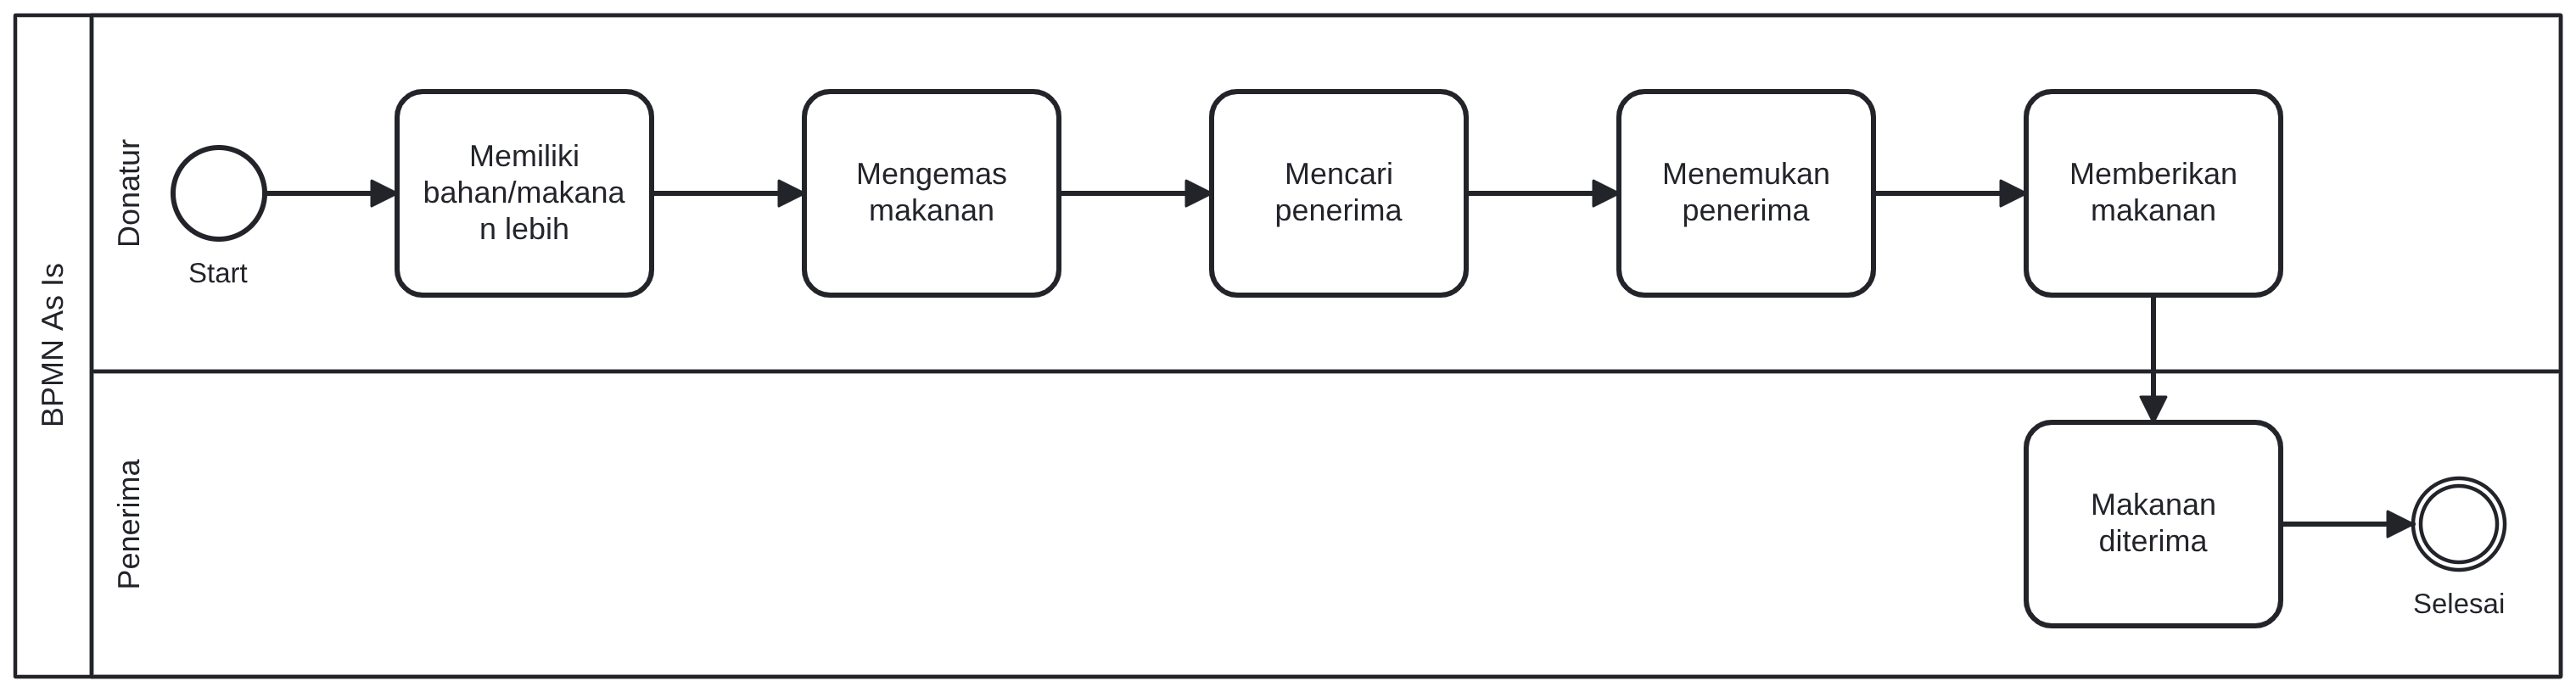
\includegraphics[width=1\textwidth]{image/bpmnAsIs.png}
    \caption{Proses Bisnis Sistem Saat Ini (BPMN As-Is)}
    \label{fig:bpmnAsIs}
\end{figure}
\begin{figure}[htbp]
    \centering
    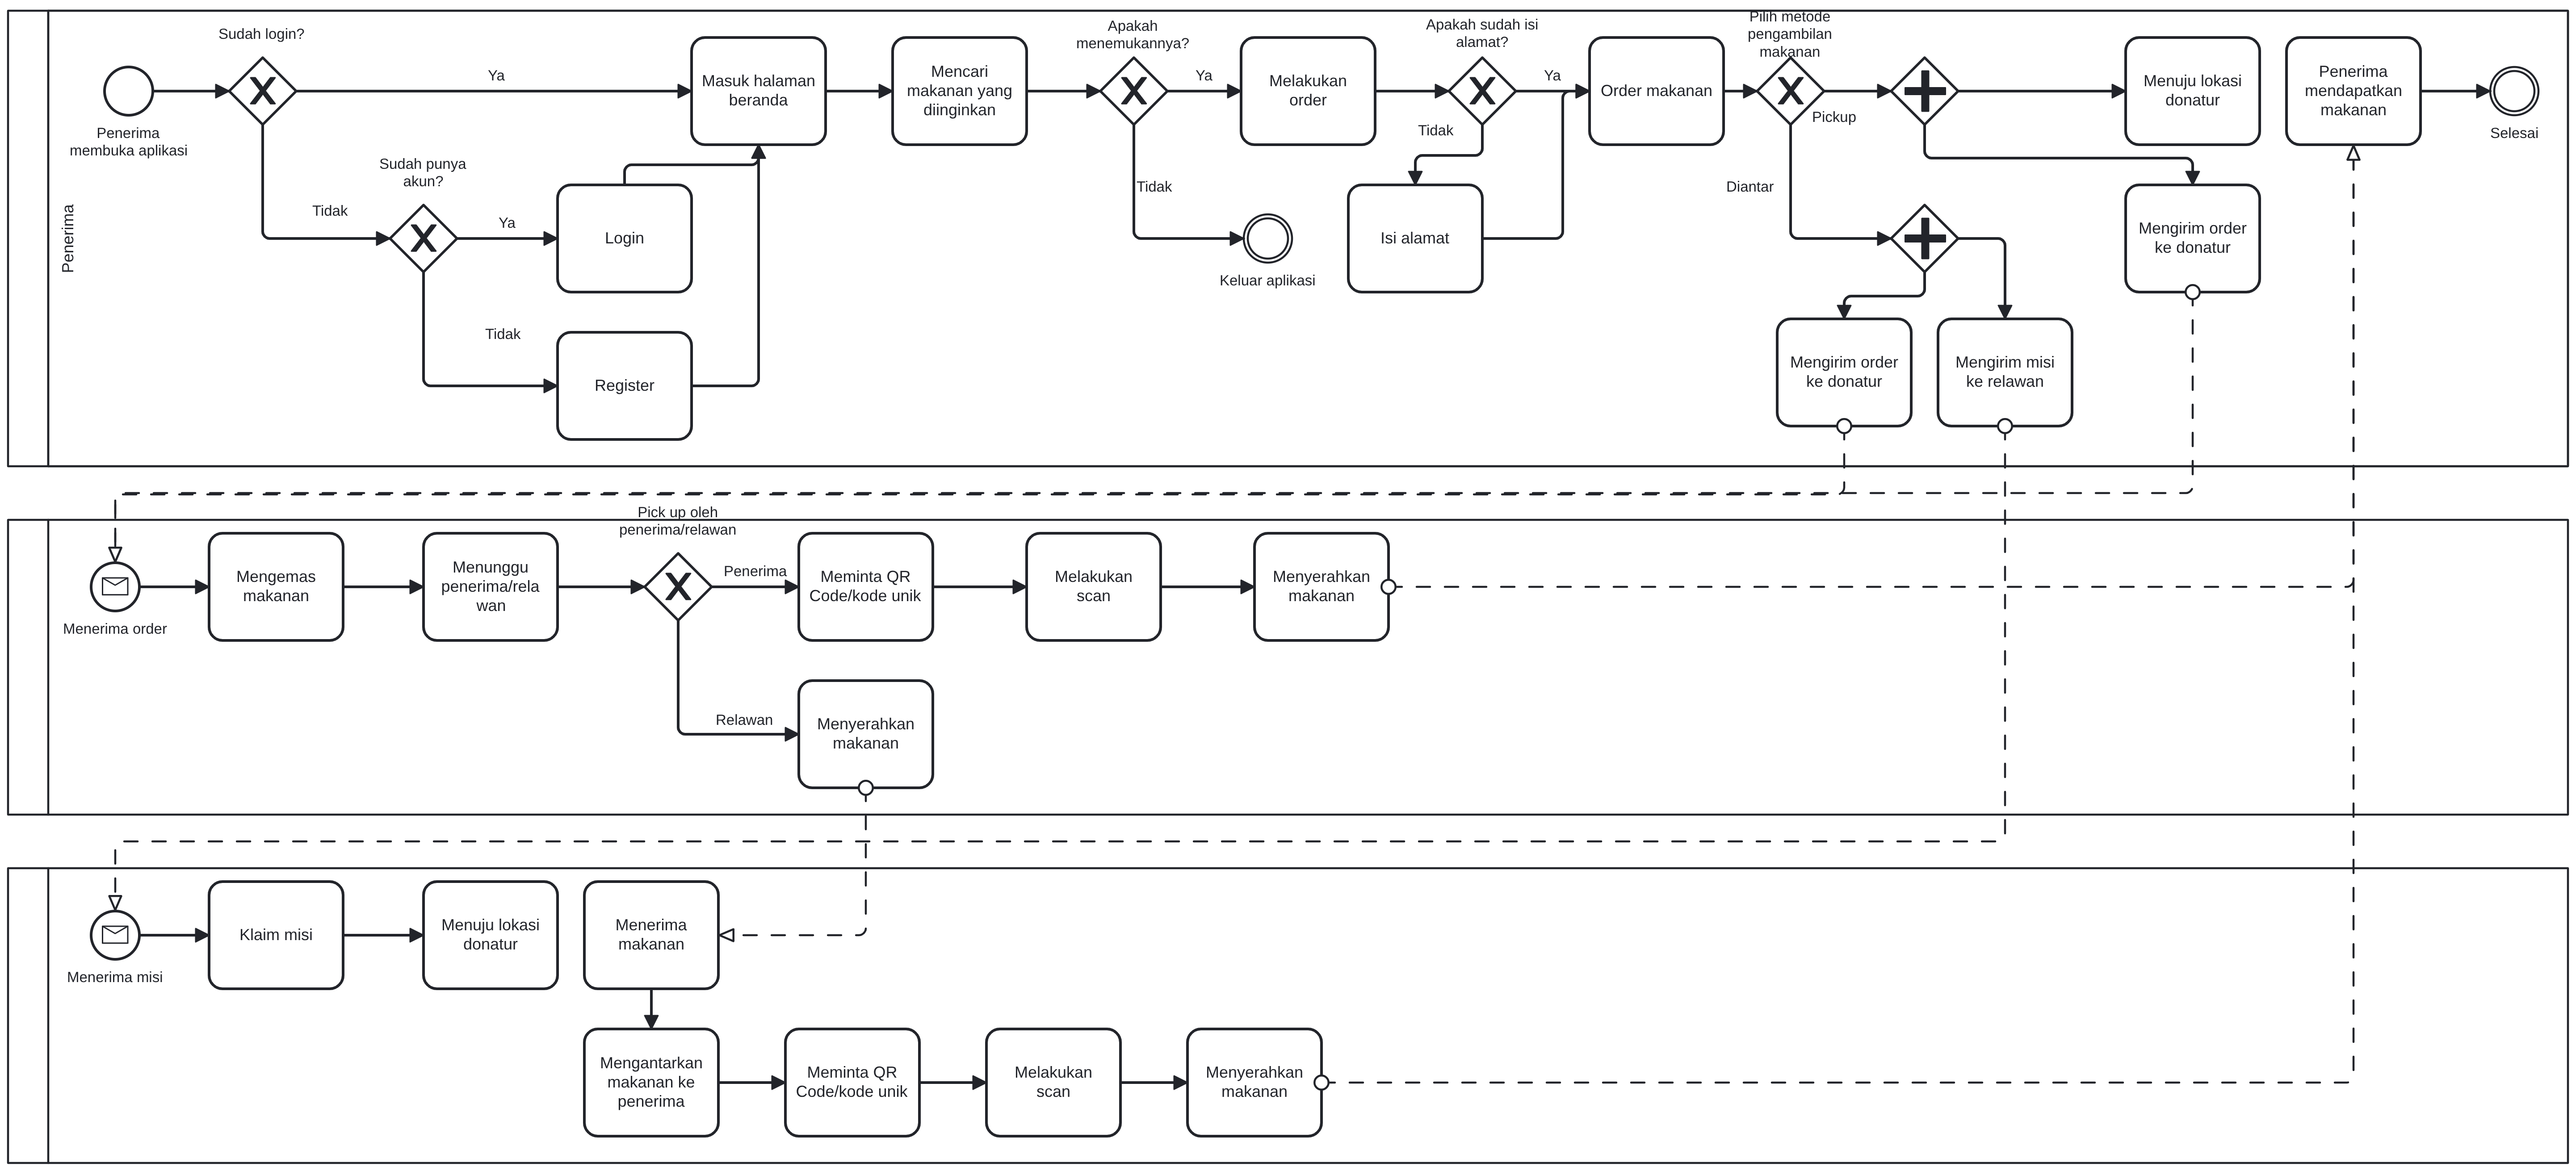
\includegraphics[width=1\textwidth]{image/bpmnToBe.png}
    \caption{Proses Bisnis Sistem Usulan (BPMN To-Be)}
    \label{fig:bpmnToBe}
\end{figure}

\newpage

\subsection{Pengalaman Pengguna}
Guna memastikan bahwa platform FoodAI Rescue yang dikembangkan dapat menyelesaikan permasalahan secara akurat dan tepat sasaran, penelitian ini menerapkan pendekatan desain berpusat pada manusia (Human-Centered Design). Pendekatan ini secara spesifik memetakan pengalaman dari target pengguna utama di lapangan—yakni pihak donatur, penerima donasi, dan relawan logistik—ketika mereka masih melakukan proses penyaluran surplus makanan secara manual atau konvensional (As-Is). Hasil pemetaan permasalahan tersebut kemudian dituangkan ke dalam tiga artefak User Experience (UX), meliputi User Persona, Empathy Map, dan User Journey Map, yang dijabarkan sebagai berikut:

\begin{figure}[htbp]
    \centering
    \includegraphics[width=1\textwidth]{image/bab2/user_persona_individu_donor.png}
    \caption{User Persona Individu Donor}
    \label{fig:userPersonaIndividuDonor}
\end{figure}
\begin{figure}[htbp]
    \centering
    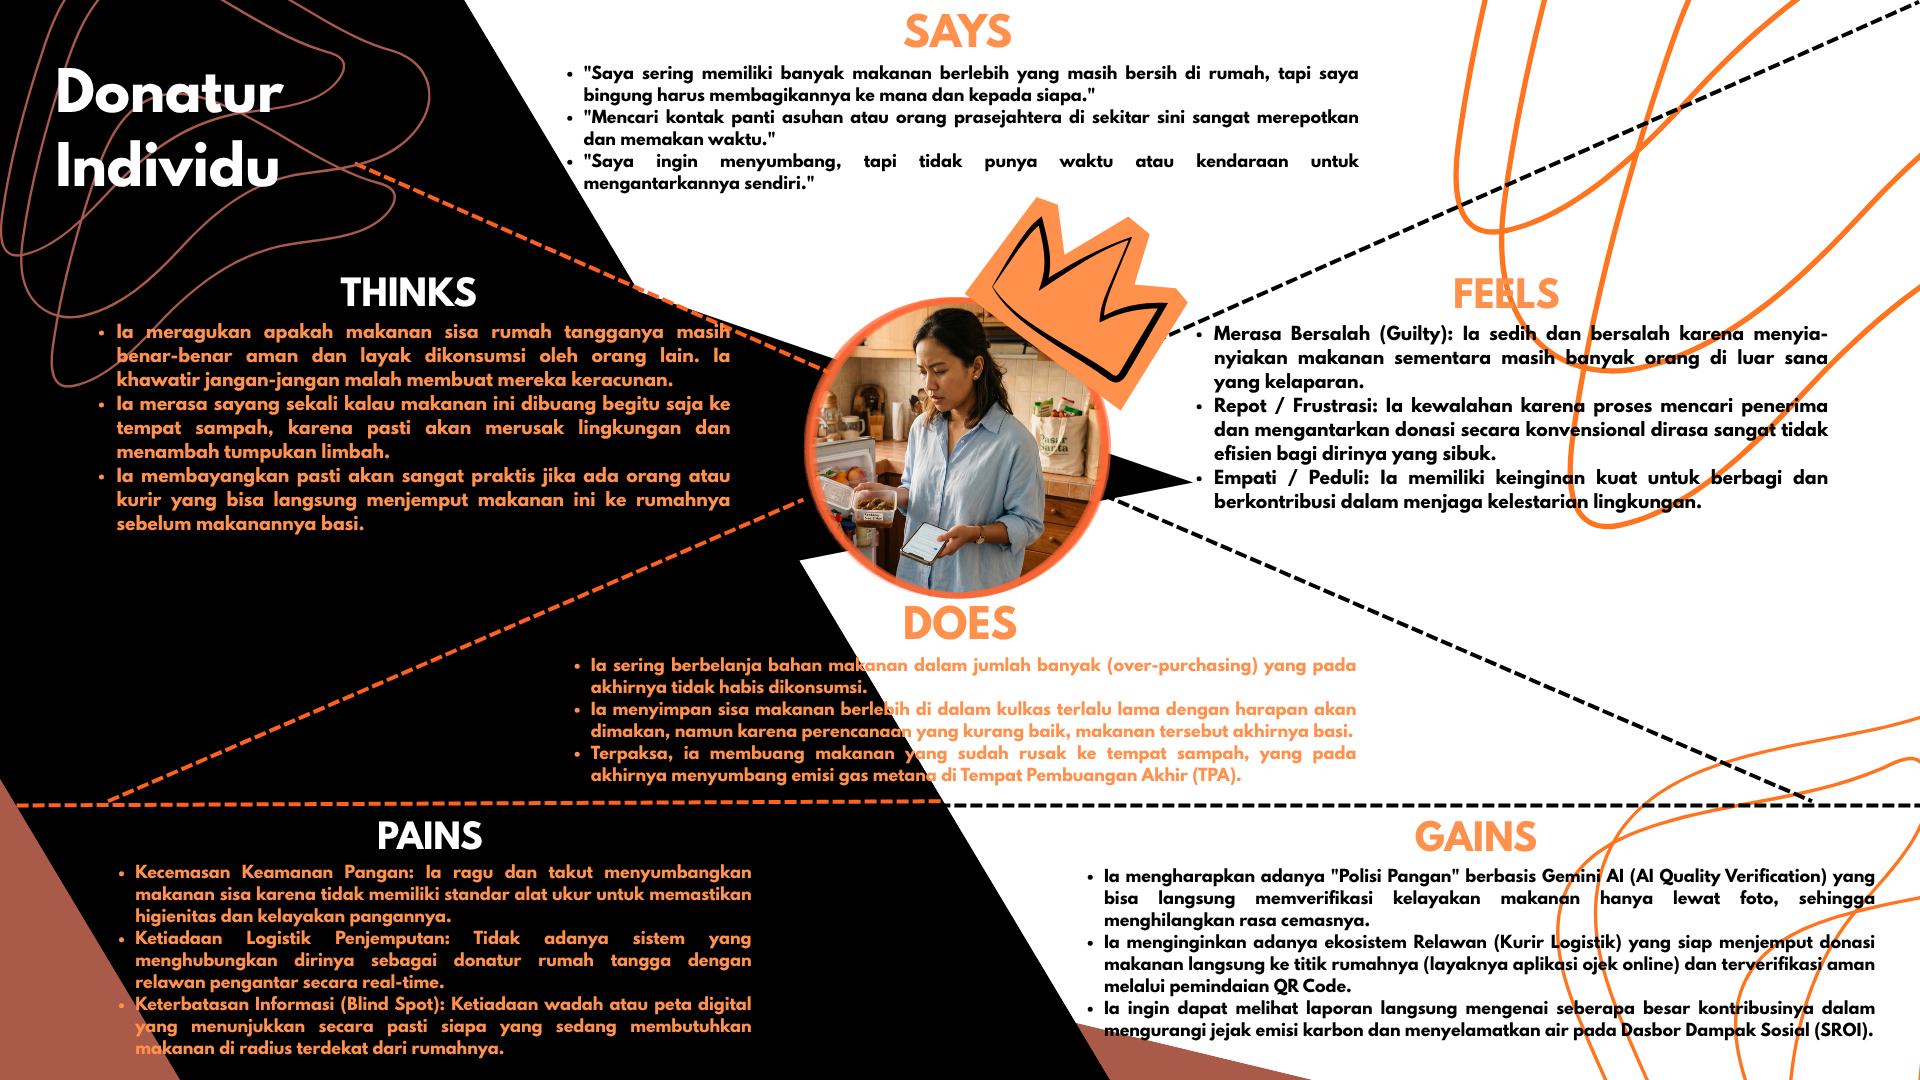
\includegraphics[width=1\textwidth]{image/bab2/segmentasi/empati_map/thinks_and_feels/donatur_individu.png}
    \caption{Empati Map Individu Donor}
    \label{fig:empatiMapIndividuDonor}
\end{figure}

\begin{figure}[htbp]
    \centering
    \includegraphics[width=1\textwidth]{image/bab2/user_persona_korporat_donor.png}
    \caption{User Persona Korporat Donor}
    \label{fig:userPersonaKorporatDonor}
\end{figure}
\begin{figure}[htbp]
    \centering
    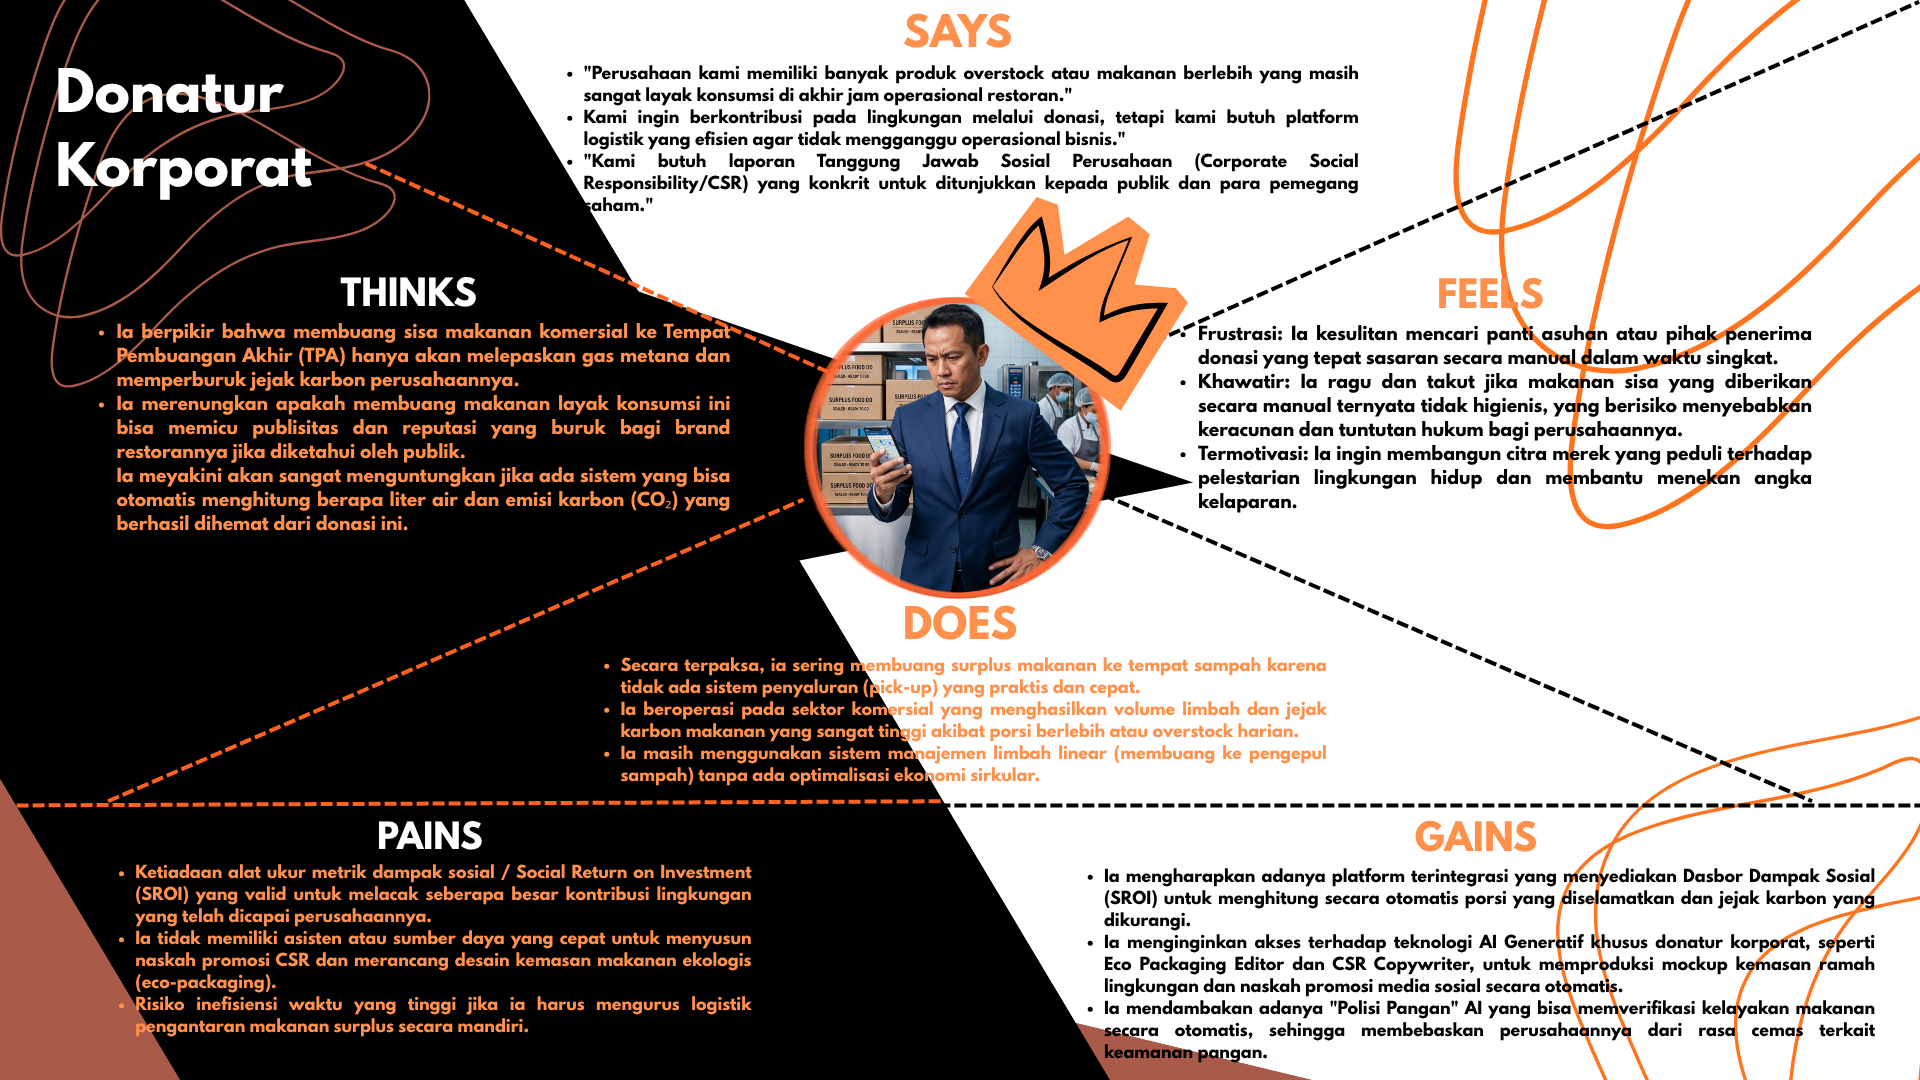
\includegraphics[width=1\textwidth]{image/bab2/segmentasi/empati_map/thinks_and_feels/donatur_korporat.png}
    \caption{Empati Map Korporat Donor}
    \label{fig:empatiMapKorporatDonor}
\end{figure}

\begin{figure}[htbp]
    \centering
    \includegraphics[width=1\textwidth]{image/bab2/user_persona_penerima.png}
    \caption{User Persona Penerima}
    \label{fig:userPersonaPenerima}
\end{figure}
\begin{figure}[htbp]
    \centering
    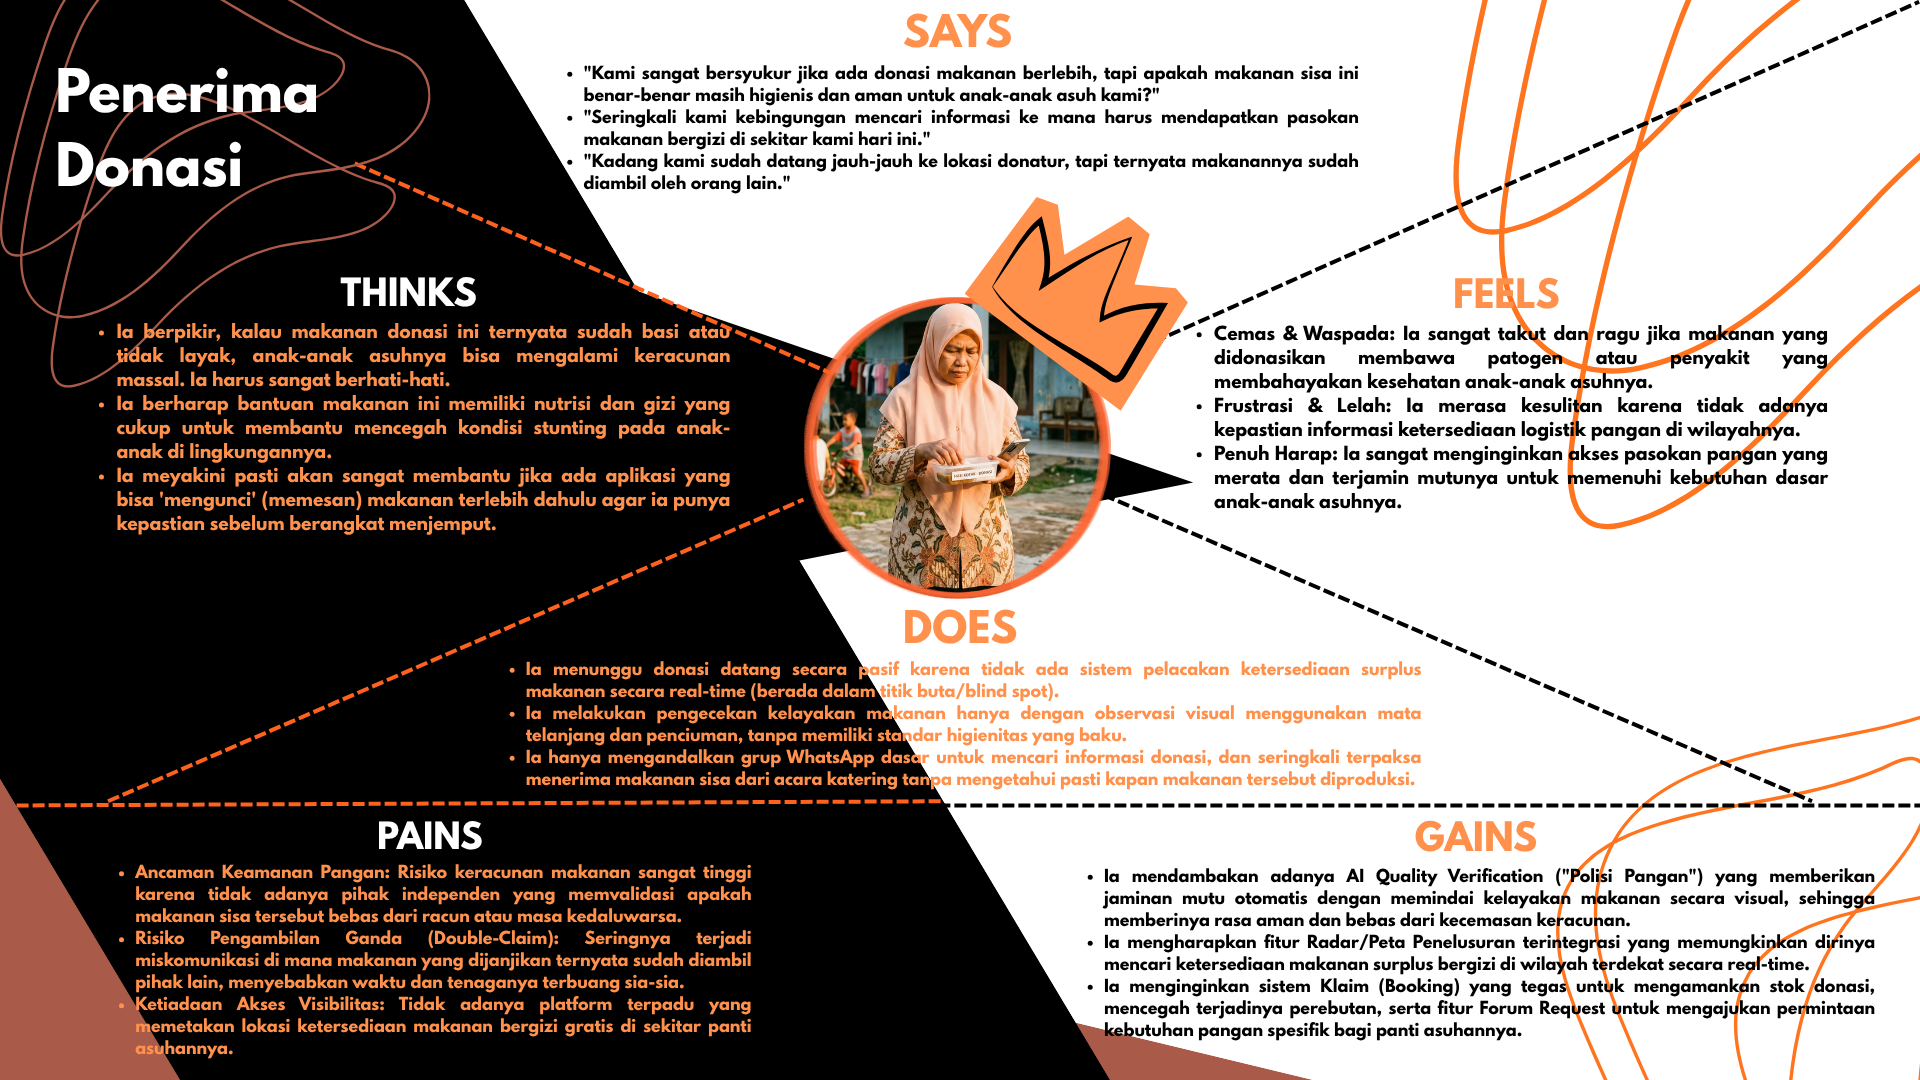
\includegraphics[width=1\textwidth]{image/bab2/segmentasi/empati_map/thinks_and_feels/penerima.png}
    \caption{Empati Map Penerima}
    \label{fig:empatiMapPenerima}
\end{figure}

\begin{figure}[htbp]
    \centering
    \includegraphics[width=1\textwidth]{image/bab2/user_persona_relawan.png}
    \caption{User Persona Relawan}
    \label{fig:userPersonaRelawan}
\end{figure}
\begin{figure}[htbp]
    \centering
    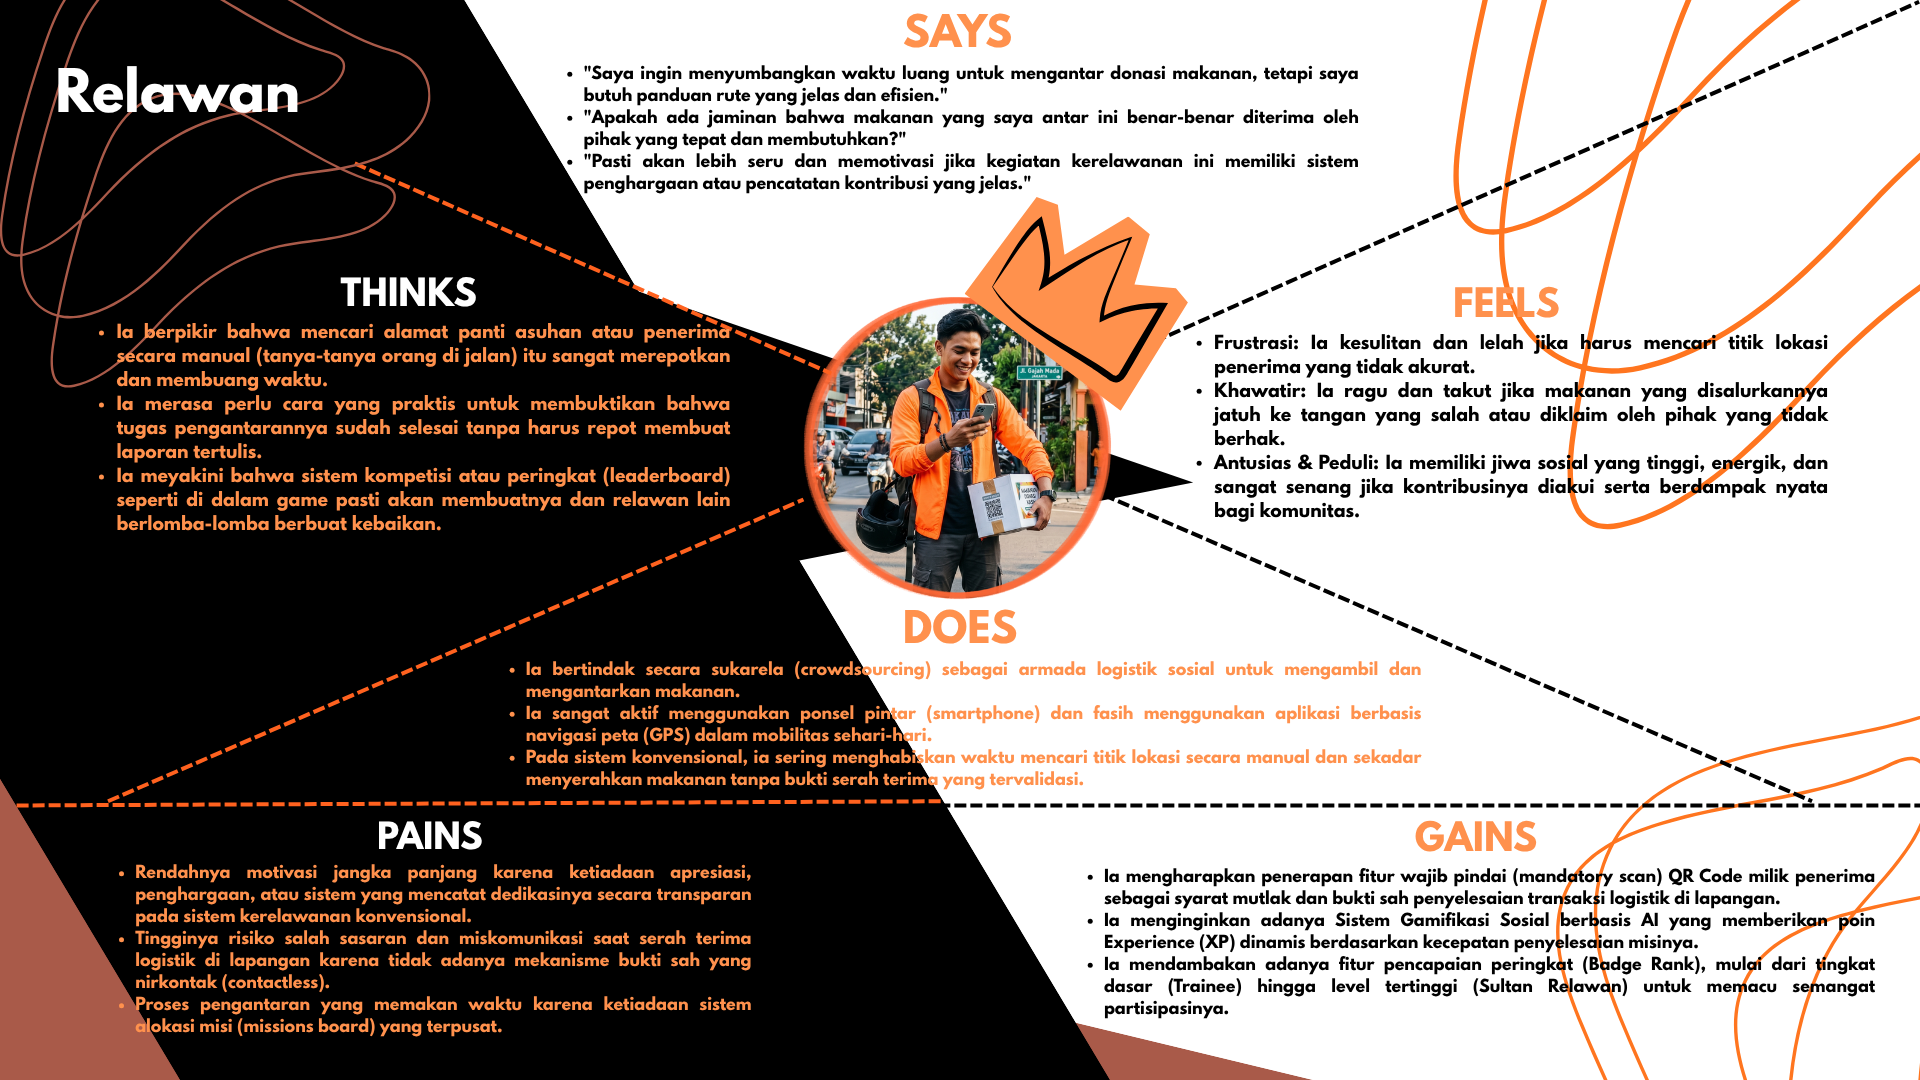
\includegraphics[width=1\textwidth]{image/bab2/segmentasi/empati_map/thinks_and_feels/relawan.png}
    \caption{Empati Map Relawan}
    \label{fig:empatiMapRelawan}
\end{figure}
\clearpage

\section{Identifikasi Aplikasi Sejenis}
Tahapan identifikasi aplikasi sejenis dilakukan guna memetakan berbagai produk atau layanan perangkat lunak di pasar (existing solutions) yang memiliki kemiripan fungsionalitas dengan sistem yang sedang diusulkan. Observasi ini ditujukan untuk menganalisis celah kelemahan (gap) dari platform pendahulu, sehingga rancangan aplikasi FoodAI Rescue mampu menghadirkan nilai tambah (value proposition) yang lebih kuat dan relevan bagi target penggunanya—seperti donatur individu, mitra korporat (HORECA), relawan, dan penerima donasi—serta selaras dengan visi instansi pengembang seperti JagoAI.

\section{Analisis Kebutuhan Sistem}
Analisis persyaratan sistem merupakan langkah esensial dalam mentransformasikan kendala operasional pada sistem manual (As-Is) serta titik keluhan (pain points) para aktor lapangan ke dalam spesifikasi teknis yang komprehensif bagi platform FoodAI Rescue. Tahapan analisis ini diklasifikasikan ke dalam tiga segmen utama, yakni pendefinisian tingkat hak akses pengguna (meliputi Donatur, Penerima, Relawan, Admin, dan SuperAdmin), pemetaan kebutuhan fungsional cerdas aplikasi, serta spesifikasi infrastruktur teknologi pendukung di sisi backend.

\subsection{Analisa Kebutuhan Fungsional}
Analisis kebutuhan fungsional menguraikan spesifikasi kapabilitas yang wajib dimiliki oleh sistem guna menjawab permasalahan pengguna di lapangan. Merujuk pada hasil observasi alur distribusi manual (As-Is) serta ekstraksi titik keluhan (pain points) dari Empathy Map dan User Journey Map, platform yang dirancang harus mampu menghadirkan solusi berupa otomatisasi verifikasi kelayakan pangan berbasis Kecerdasan Buatan (AI), pencocokan donasi secara real-time, serta rekapitulasi pelaporan dampak lingkungan (SROI) secara digital. Oleh karena itu, fungsionalitas yang akan diimplementasikan pada ekosistem FoodAI Rescue diklasifikasikan ke dalam enam modul utama berikut

\subsection{Analisa Kebutuhan Dukungan Sistem}
Agar seluruh fungsionalitas aplikasi dapat beroperasi secara optimal, responsif, dan terotomatisasi, platform FoodAI Rescue tidak dapat hanya mengandalkan antarmuka pengguna ( frontend ) saja. Platform ini menuntut adanya dukungan arsitektur sistem di sisi backend yang tangguh. Secara konseptual, infrastruktur di belakang layar ini diklasifikasikan ke dalam tiga pilar kebutuhan operasional utama: pemenuhan fungsionalitas konten (manajemen donasi dan pengguna), ketersediaan layanan integrasi (API services), serta infrastruktur teknologi pendukung Kecerdasan Buatan (seperti integrasi Google Gemini Vision API) yang menjadi motor penggerak inovasi sistem.

\section{Kinerja Sistem }
Kinerja sistem merepresentasikan standar minimum dan tolok ukur (benchmark) yang diterapkan guna memastikan seluruh ekosistem aplikasi FoodAI Rescue, khususnya pada Modul Konfigurasi Pusat (Admin) dan Dasbor Dampak Sosial (SROI), mampu beroperasi selaras dengan spesifikasi dan perancangan fungsionalnya. Proses evaluasi kinerja dalam pengembangan platform ini dititikberatkan pada empat parameter fundamental, meliputi: fungsionalitas antarmuka perangkat lunak, keandalan serta stabilitas jalur komunikasi data (terutama integrasi Google Gemini API), tingkat responsivitas keamanan sistem, dan metrik kecepatan muat halaman (page load). Ruang lingkup pengukuran kinerja ini tidak melibatkan pengujian ketahanan perangkat keras fisik (hardware) di lapangan, melainkan dibatasi secara ketat pada domain rekayasa perangkat lunak dengan rincian standar pengujian sebagai berikut:
% \chapter{PERSYARATAN SISTEM }

\label{chapter:PERSYARATAN SISTEM}

\section{Deskripsi Pengguna}
Target pengguna utama dari aplikasi Food AI Rescue (FAR) secara umum adalah seluruh entitas yang terlibat dalam ekosistem pengelolaan surplus makanan, rantai pasok logistik sosial, dan penerima manfaat di tingkat komunitas. Sistem ini memfasilitasi kolaborasi multi-pihak yang dirancang agar ramah pengguna (user-friendly), baik bagi masyarakat awam, pelaku usaha, maupun tim manajerial. Untuk memetakan kebutuhan sistem, pengguna aplikasi ini didetailkan ke dalam segmentasi dan peran (role) sebagai berikut:

% \subsection{Segmentasi Pengguna}

\begin{figure}[htbp]
    \centering
    \includegraphics[width=1\textwidth]{image/bab2/segmentasi.png}
    \caption{Segmentasi Pengguna Food AI Rescue}
    \label{fig:segmentasi}
\end{figure}

\begin{enumerate}
    \item \textbf{Donatur Individu}
    \begin{itemize}
        \item \textbf{Segmen/Profil}: Masyarakat perorangan atau pelaku usaha skala mikro yang memiliki kelebihan produksi makanan dalam jumlah kecil (skala rumah tangga).
        \item \textbf{Peranan dan Hak Akses Utama}: Memiliki hak untuk mengunggah data makanan surplus, memperbarui status ketersediaan (\textit{inventory}), serta melakukan serah terima secara langsung. Pada saat serah terima menggunakan fitur Janji Temu (COD), pengguna wajib memindai QR Code milik Penerima sebagai bukti distribusi yang sah. Selain itu, donatur memiliki akses untuk memantau Dasbor Dampak Sosial (SROI) yang memuat laporan total porsi terselamatkan dan estimasi pengurangan emisi jejak karbon (CO$_2$).
        \item \textbf{Hak Akses AI}: Memiliki akses ke fitur bawaan AI \textit{Quality Verification}. Sebelum donasi dipublikasikan, donatur wajib memindai foto makanan menggunakan kamera AI ini guna memastikan kelayakan fisik dan higienitas visual. Selain itu, donatur juga dapat memindai (\textit{scan}) bahan makanan untuk mendapatkan rekomendasi resep masakan dari sistem.
    \end{itemize}
    \item \textbf{Donatur Kelompok/Korporat (Mitra Penyedia)}
    \begin{itemize}
        \item \textbf{Segmen/Profil}: Pelaku bisnis skala besar di sektor \textit{Hospitality, Restaurant, and Cafe} (HORECA) seperti restoran, hotel, atau usaha katering berskala komersial.
        \item \textbf{Peranan dan Hak Akses Utama}: Memiliki peranan dan hak akses operasional yang sama persis dengan Donatur Individu, mulai dari siklus manajemen distribusi (unggah surplus, update \textit{inventory}, pindai QR serah terima) hingga pemantauan laporan di Dasbor Dampak Sosial (SROI).
        \item \textbf{Hak Akses Khusus (Spesial) AI}: Sebagai nilai tambah (\textit{value}) untuk mendukung kampanye pemasaran dan \textit{Corporate Social Responsibility} (CSR) perusahaan, donatur tingkat kelompok/korporat dibekali hak istimewa terhadap dua modul AI generatif eksklusif, yaitu:
        \begin{itemize}
            \item \textbf{\textit{Generate Image} Kemasan}: Hak spesial untuk menghasilkan gambar desain prototipe bungkus atau kemasan makanan.
            \item \textbf{\textit{Generate} Konten Media Sosial}: Hak spesial untuk secara otomatis menghasilkan gambar visual desain (lengkap dengan stiker verifikasi AI dan logo perusahaan) sekaligus memproduksi konten tulisan (\textit{copywriting}) promosi yang siap diunggah ke platform media sosial.
        \end{itemize}
    \end{itemize}
    \item \textbf{Penerima (Mitra Penerima)}
    \begin{itemize}
        \item \textbf{Segmen/Profil}: Masyarakat di kawasan rentan pangan, panti asuhan, dewan kemakmuran masjid (DKM), atau warga prasejahtera di desa sasaran yang membutuhkan bantuan makanan.
        \item \textbf{Peranan dan Hak Akses}: Memiliki akses untuk mencari menu makanan terdekat, melakukan proses klaim (booking) guna mengunci stok dan mencegah insiden pengambilan ganda (double-claim) oleh pihak lain, memilih metode pengambilan, dan menyajikan QR Code miliknya untuk dipindai saat makanan tiba.
        \item \textbf{Hak Akses Khusus AI}: Penerima diberikan akses ke fitur AI \textit{Quality Verification} untuk memindai kelayakan fisik dan higienitas visual makanan sebelum dikonsumsi, fitur Forum Request untuk memublikasikan kebutuhan pangan spesifik, serta memberikan ulasan (\textit{feedback}).
    \end{itemize}
    \item \textbf{Relawan}
    \begin{itemize}
        \item \textbf{Segmen/Profil}: Pemuda lokal, warga desa, atau masyarakat umum yang bertindak secara sukarela (\textit{crowdsourcing}) sebagai armada logistik sosial.
        \item \textbf{Peranan dan Hak Akses}: Mengakses daftar misi pengantaran, melakukan penjemputan makanan dari lokasi Donatur, dan mengantarkannya secara langsung ke titik lokasi Penerima. Relawan memegang otoritas validasi lapangan dengan hak akses wajib pindai (\textit{mandatory scan}) QR Code milik Penerima sebagai syarat mutlak penyelesaian transaksi distribusi.
    \end{itemize}
    \item \textbf{Admin Pengelola}
    \begin{itemize}
        \item \textbf{Segmen/Profil}: Tim manajerial dan pengawas operasional harian yang bertugas mengelola sistem secara administratif di tingkat komunitas.
        \item \textbf{Peranan dan Hak Akses}: Memiliki hak akses dashboard admin untuk memverifikasi keabsahan pendaftaran akun baru secara manual, membekukan atau memblokir akun yang terbukti melakukan penyalahgunaan, menindaklanjuti laporan negatif, serta memantau Dasbor Statistik makro yang menampilkan peta panas (\textit{heatmap}) sebaran wilayah donasi dan kalkulasi SROI keseluruhan.
    \end{itemize}
    \item \textbf{Super Admin}
    \begin{itemize}
        \item \textbf{Segmen/Profil}: Pengembang sistem (Tim IT / Programmer).
        \item \textbf{Peranan dan Hak Akses}: Memiliki tingkat hak akses paling tinggi dan menyeluruh pada sisi \textit{backend} aplikasi. Super Admin bertugas untuk melakukan pemeliharaan server secara berkala (\textit{maintenance}), menangani perbaikan apabila terdapat laporan \textit{bug} dari sistem, dan menjaga stabilitas basis data secara penuh.
    \end{itemize}
\end{enumerate}

\newpage

\section{Gambaran Sistem Saat Ini}
Gambaran sistem yang berjalan saat ini (As-Is) pada ekosistem penyaluran donasi surplus makanan di masyarakat masih sepenuhnya mengandalkan metode konvensional secara manual dan tidak terstruktur. Hingga saat ini, belum ada satu pun aplikasi khusus atau sistem terintegrasi yang memfasilitasi tata kelola operasional logistik donasi pangan secara digital yang disertai dengan jaminan standar keamanan mutu. Startup JagoAI sebagai pihak inovator juga belum memiliki platform pusat kendali (command center) untuk memonitor aktivitas donasi, memvalidasi kelayakan makanan secara otomatis, serta melacak pergerakan relawan kurir secara terpusat.
% \\
% Berdasarkan hasil observasi di lapangan, seluruh pencatatan data ketersediaan surplus makanan dan riwayat penyalurannya masih tidak terdokumentasi dengan baik atau hanya dicatat secara manual. Selain itu, proses pengecekan kelayakan dan keamanan pangan hanya mengandalkan observasi visual dengan mata telanjang oleh pihak donatur tanpa standar higienitas yang baku. Satu-satunya perangkat lunak yang umum digunakan dalam ekosistem penyaluran donasi saat ini hanyalah aplikasi pesan instan pihak ketiga (seperti grup WhatsApp), yang sekadar dimanfaatkan sebagai sarana komunikasi dasar, bukan sebagai sistem manajemen logistik terpadu maupun penyimpan basis data (database). Ketiadaan sistem yang terintegrasi ini menyebabkan rantai informasi penjemputan sering terputus, tingginya risiko ancaman kesehatan bagi penerima akibat kelalaian manusia (human error) dalam memvalidasi makanan, serta lambatnya proses distribusi yang berujung pada membusuknya makanan sebelum disalurkan sehingga tetap berakhir menjadi tumpukan limbah makanan (food waste).
\subsection{Analisis Proses Bisnis}
Pada sistem manual, proses berbagi makanan berlebih berjalan secara sporadis, linear, dan tidak terstruktur. Ketika rumah tangga, penyelenggara acara, atau pelaku industri (seperti restoran dan hotel) memiliki surplus makanan, mereka harus mencari sendiri fasilitas sosial atau individu yang membutuhkan secara tatap muka atau melalui pesan singkat yang terbatas. Ketiadaan rantai pasok logistik yang terpusat ini menyebabkan waktu terbuang percuma hanya untuk mencari siapa yang bersedia menerima makanan tersebut. Akibatnya, banyak makanan yang awalnya masih layak konsumsi menjadi basi atau kedaluwarsa di tengah jalan, sehingga pada akhirnya tetap berujung dibuang ke Tempat Pembuangan Akhir (TPA) dan memicu masalah emisi gas rumah kaca.

\begin{figure}[htbp]
    \centering
    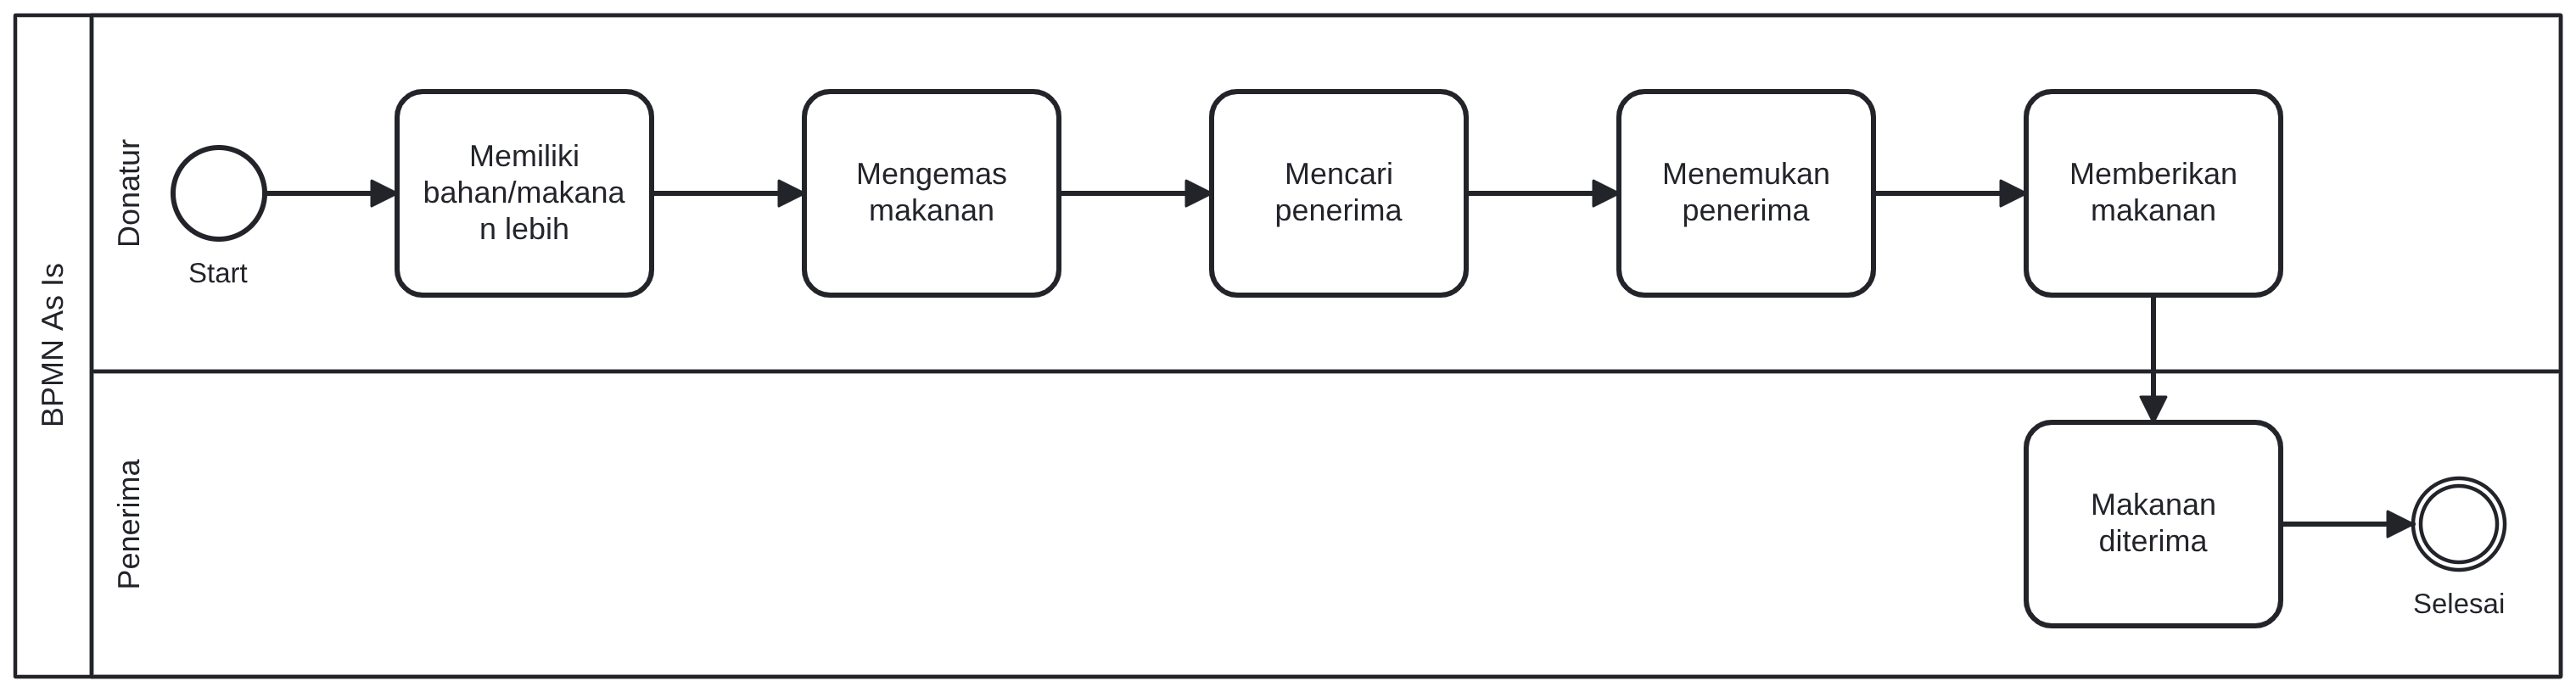
\includegraphics[width=1\textwidth]{image/bpmnAsIs.png}
    \caption{Proses Bisnis Sistem Saat Ini (BPMN As-Is)}
    \label{fig:bpmnAsIs}
\end{figure}
\begin{figure}[htbp]
    \centering
    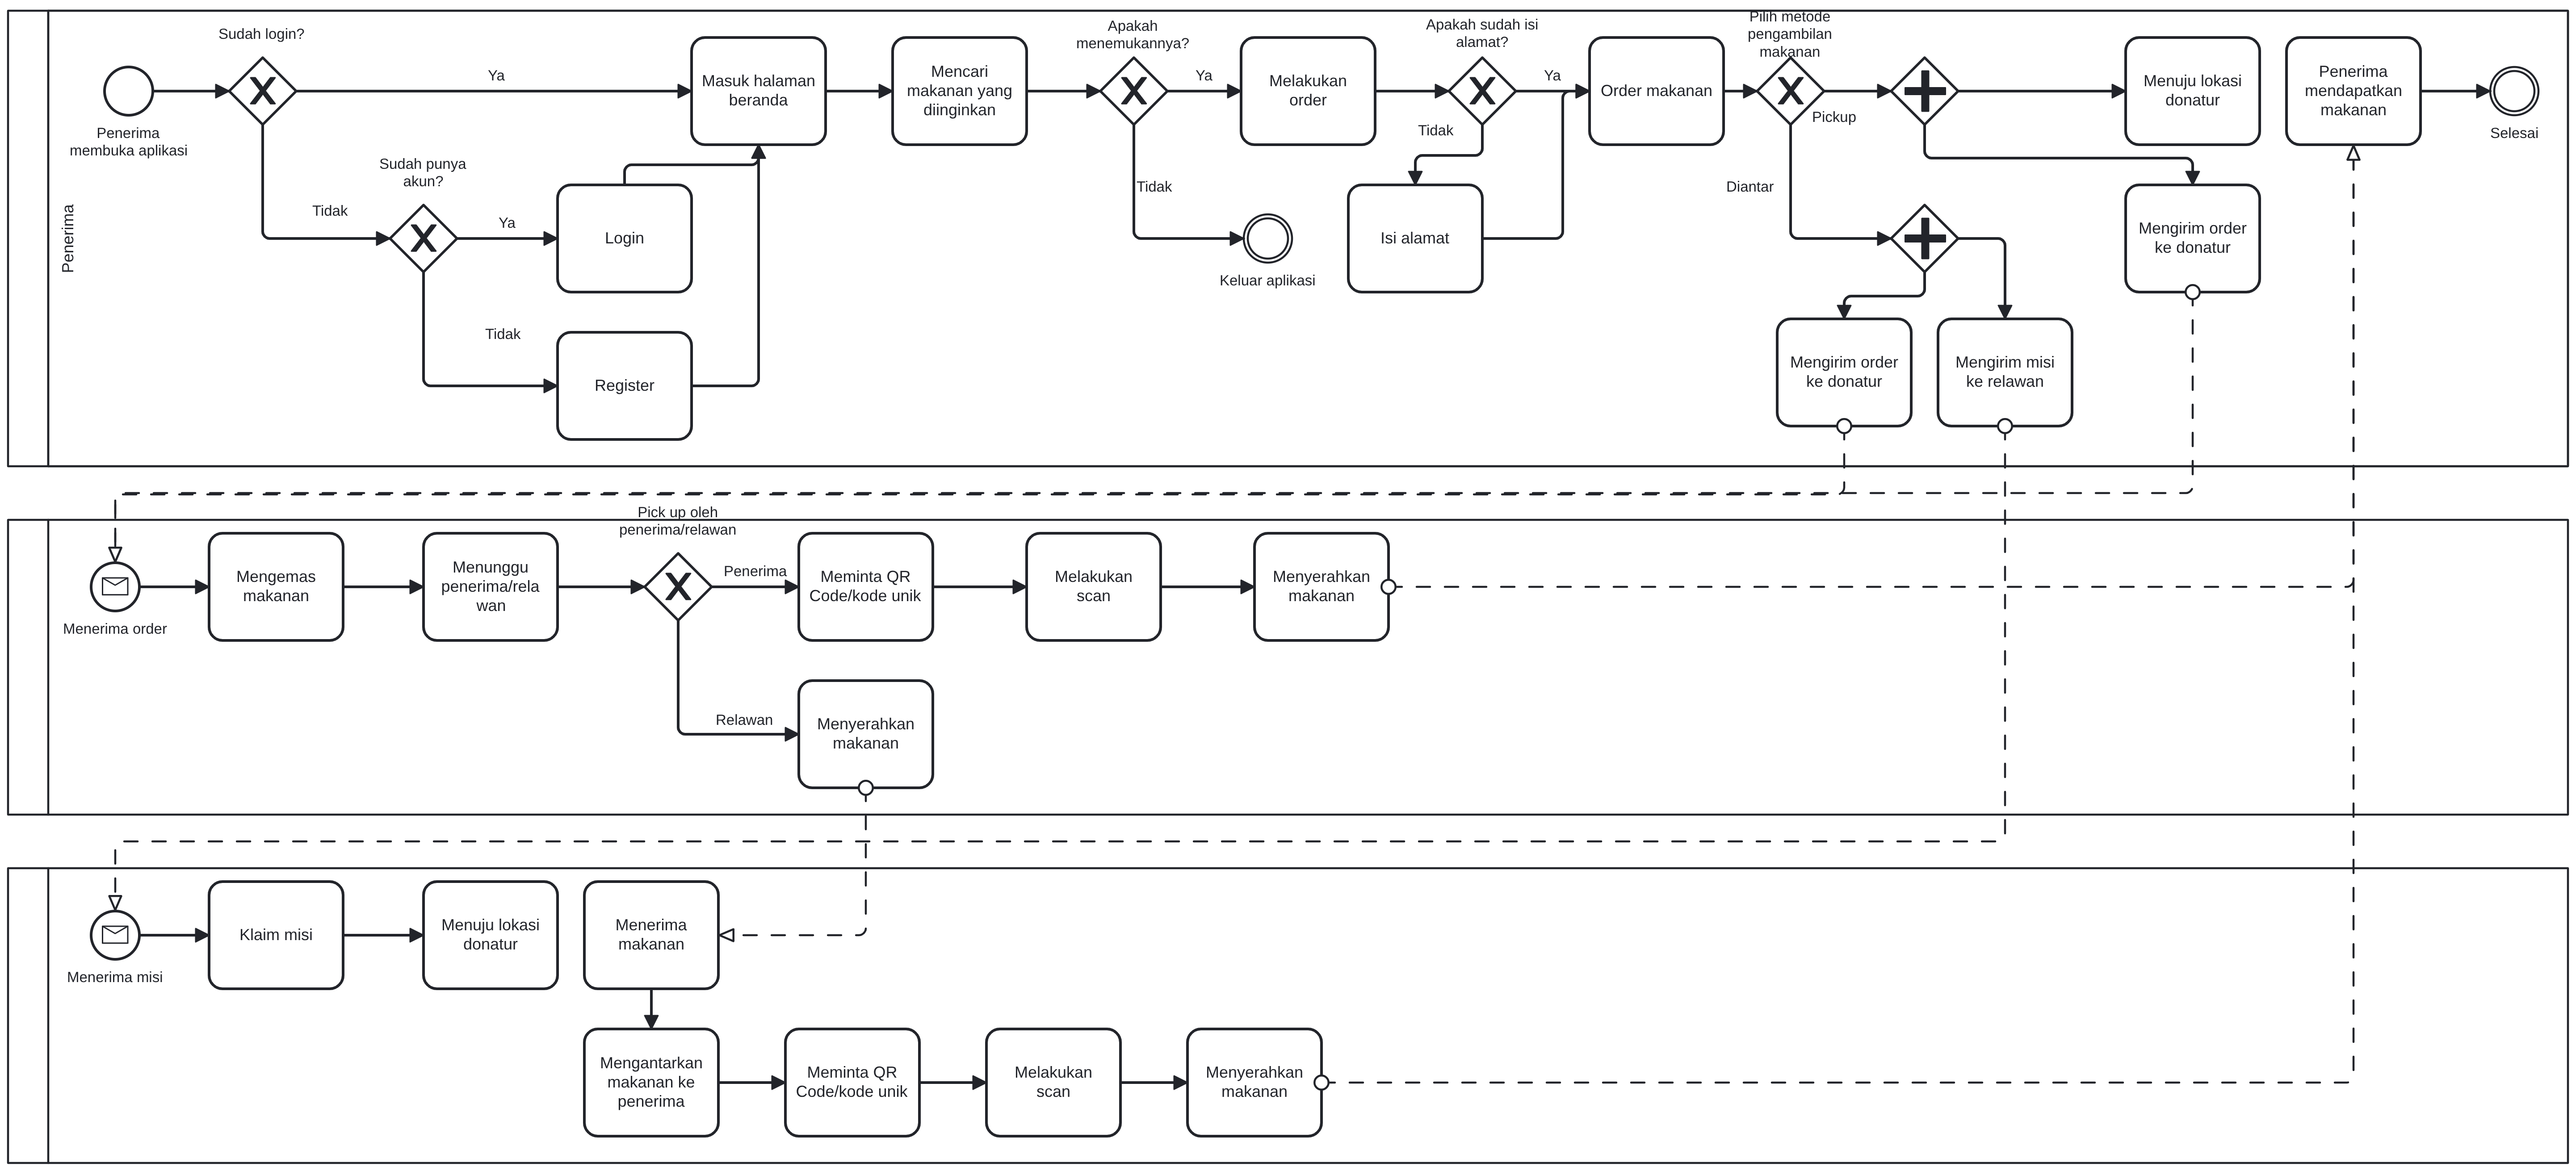
\includegraphics[width=1\textwidth]{image/bpmnToBe.png}
    \caption{Proses Bisnis Sistem Usulan (BPMN To-Be)}
    \label{fig:bpmnToBe}
\end{figure}

\newpage

\subsection{Pengalaman Pengguna}
Guna memastikan bahwa platform FoodAI Rescue yang dikembangkan dapat menyelesaikan permasalahan secara akurat dan tepat sasaran, penelitian ini menerapkan pendekatan desain berpusat pada manusia (Human-Centered Design). Pendekatan ini secara spesifik memetakan pengalaman dari target pengguna utama di lapangan—yakni pihak donatur, penerima donasi, dan relawan logistik—ketika mereka masih melakukan proses penyaluran surplus makanan secara manual atau konvensional (As-Is). Hasil pemetaan permasalahan tersebut kemudian dituangkan ke dalam tiga artefak User Experience (UX), meliputi User Persona, Empathy Map, dan User Journey Map, yang dijabarkan sebagai berikut:

\begin{figure}[htbp]
    \centering
    \includegraphics[width=1\textwidth]{image/bab2/user_persona_individu_donor.png}
    \caption{User Persona Individu Donor}
    \label{fig:userPersonaIndividuDonor}
\end{figure}
\begin{figure}[htbp]
    \centering
    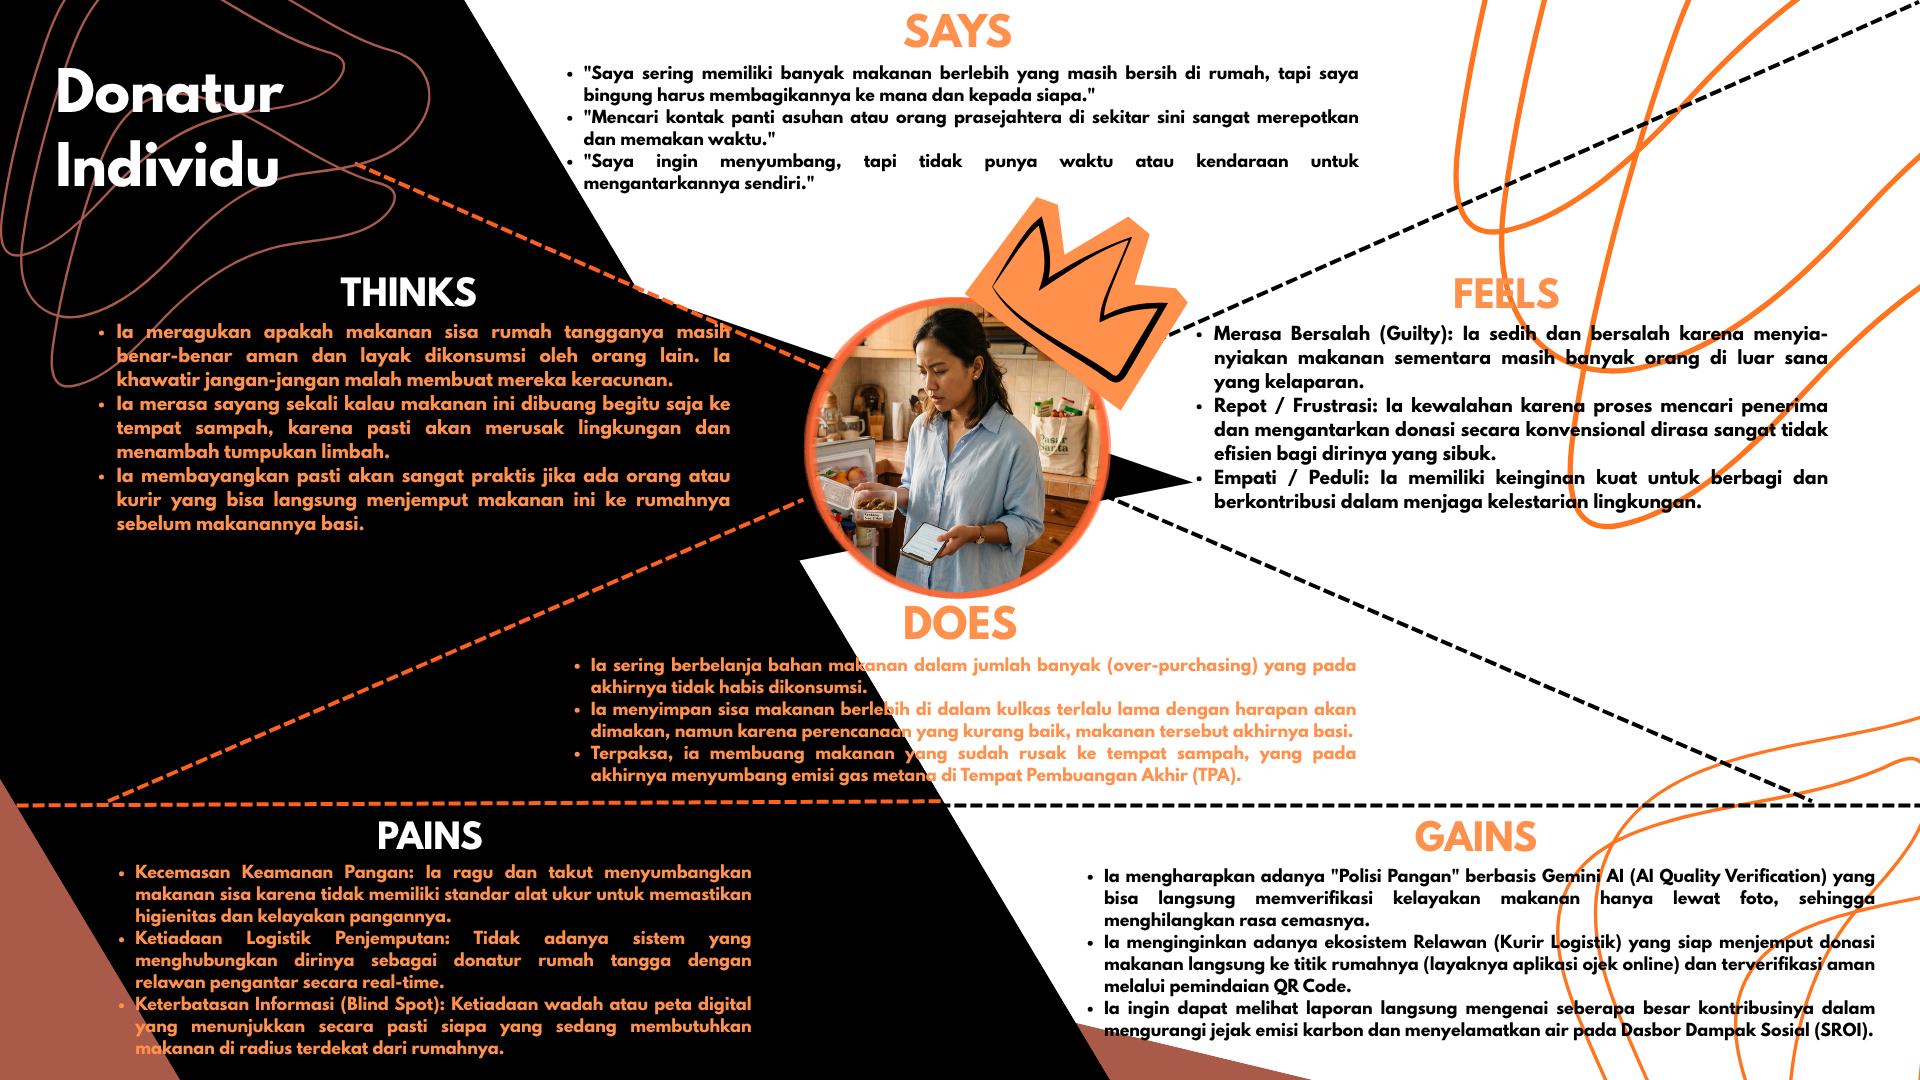
\includegraphics[width=1\textwidth]{image/bab2/segmentasi/empati_map/thinks_and_feels/donatur_individu.png}
    \caption{Empati Map Individu Donor}
    \label{fig:empatiMapIndividuDonor}
\end{figure}

\begin{figure}[htbp]
    \centering
    \includegraphics[width=1\textwidth]{image/bab2/user_persona_korporat_donor.png}
    \caption{User Persona Korporat Donor}
    \label{fig:userPersonaKorporatDonor}
\end{figure}
\begin{figure}[htbp]
    \centering
    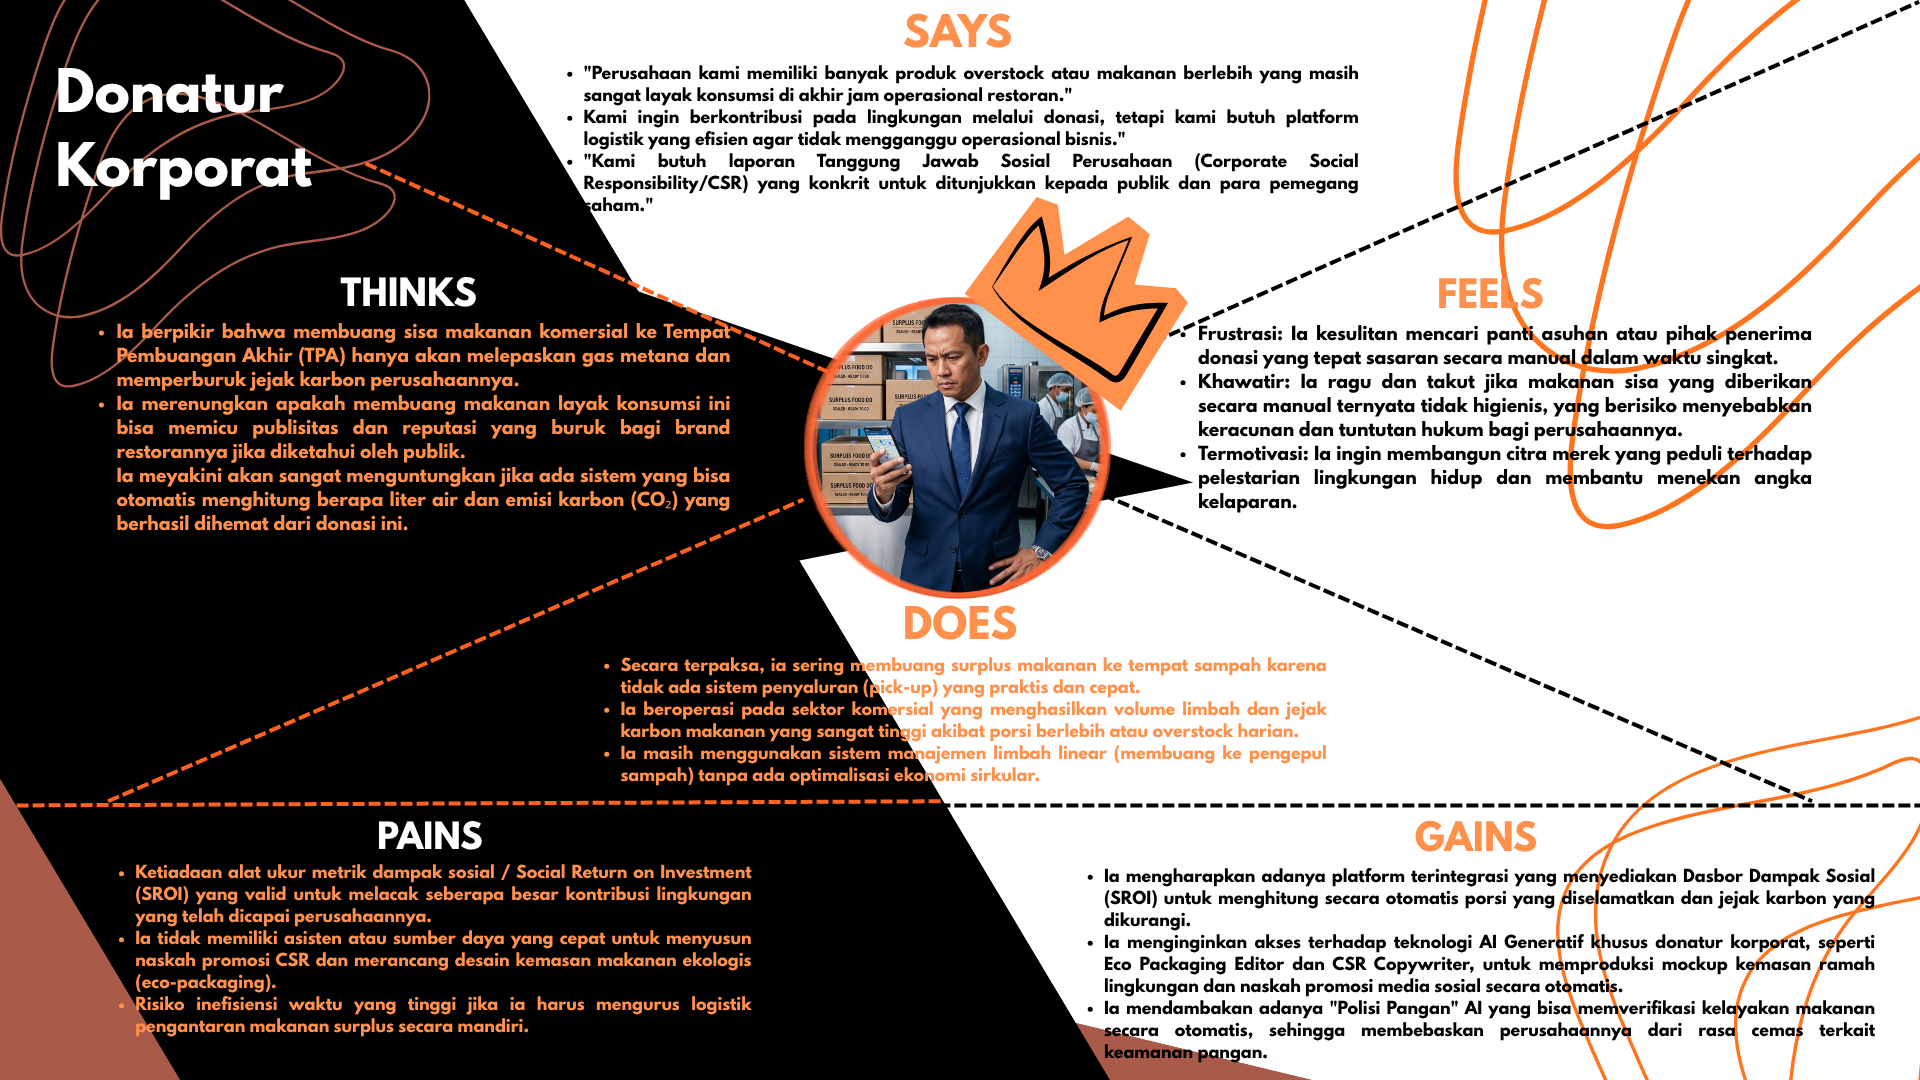
\includegraphics[width=1\textwidth]{image/bab2/segmentasi/empati_map/thinks_and_feels/donatur_korporat.png}
    \caption{Empati Map Korporat Donor}
    \label{fig:empatiMapKorporatDonor}
\end{figure}

\begin{figure}[htbp]
    \centering
    \includegraphics[width=1\textwidth]{image/bab2/user_persona_penerima.png}
    \caption{User Persona Penerima}
    \label{fig:userPersonaPenerima}
\end{figure}
\begin{figure}[htbp]
    \centering
    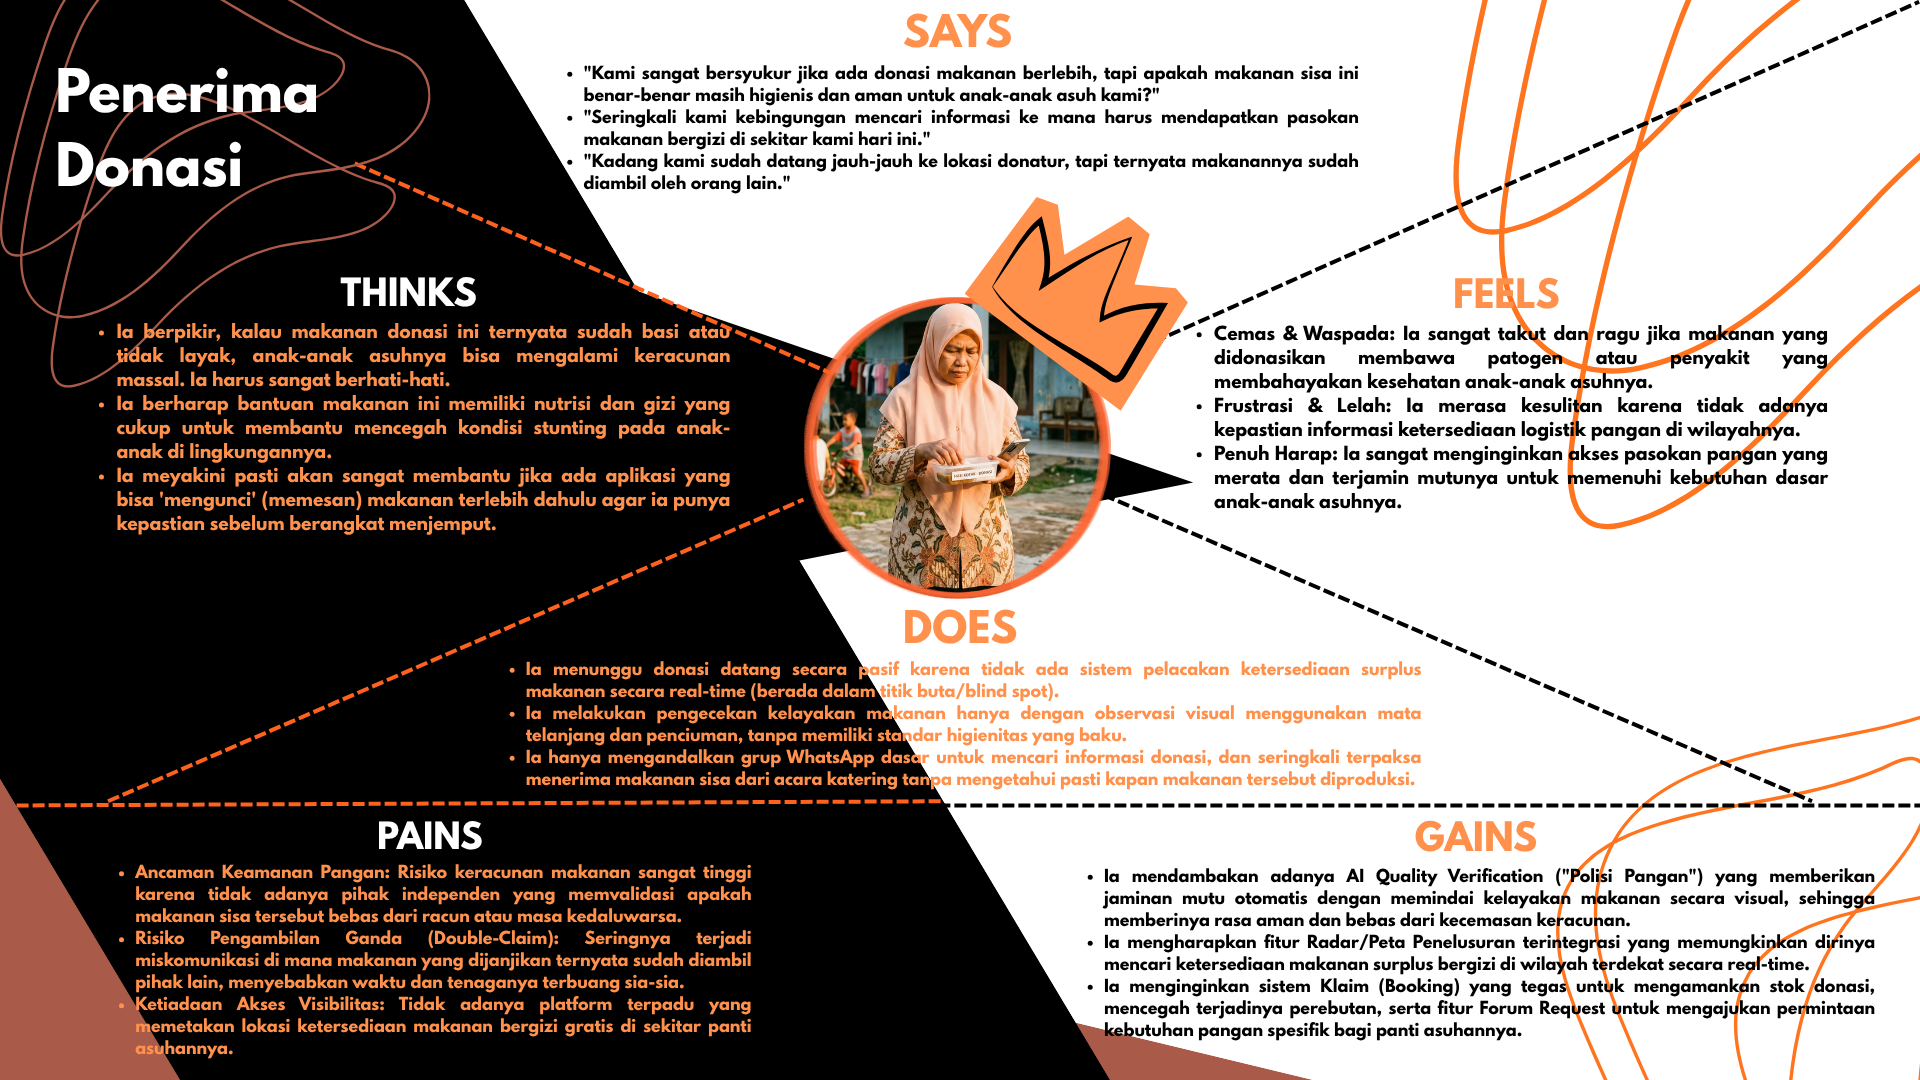
\includegraphics[width=1\textwidth]{image/bab2/segmentasi/empati_map/thinks_and_feels/penerima.png}
    \caption{Empati Map Penerima}
    \label{fig:empatiMapPenerima}
\end{figure}

\begin{figure}[htbp]
    \centering
    \includegraphics[width=1\textwidth]{image/bab2/user_persona_relawan.png}
    \caption{User Persona Relawan}
    \label{fig:userPersonaRelawan}
\end{figure}
\begin{figure}[htbp]
    \centering
    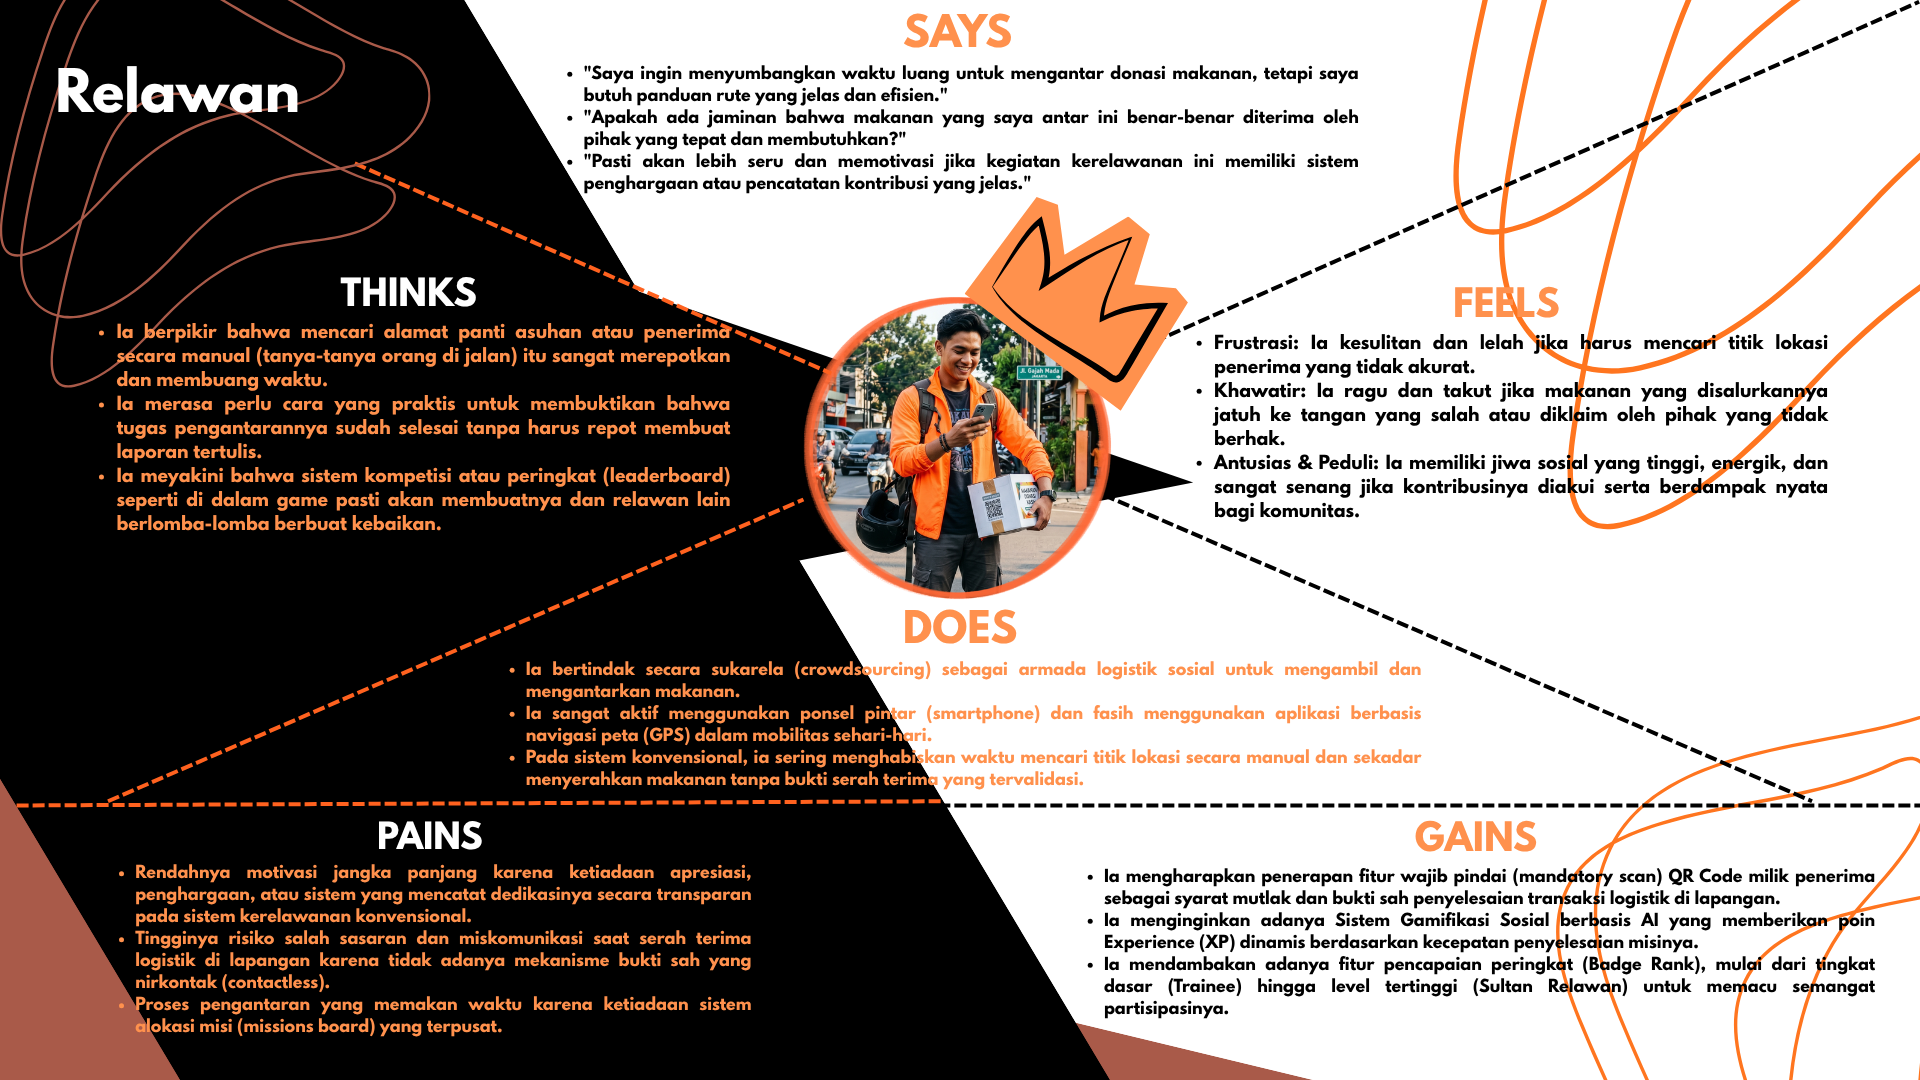
\includegraphics[width=1\textwidth]{image/bab2/segmentasi/empati_map/thinks_and_feels/relawan.png}
    \caption{Empati Map Relawan}
    \label{fig:empatiMapRelawan}
\end{figure}
\clearpage

\section{Identifikasi Aplikasi Sejenis}
Tahapan identifikasi aplikasi sejenis dilakukan guna memetakan berbagai produk atau layanan perangkat lunak di pasar (existing solutions) yang memiliki kemiripan fungsionalitas dengan sistem yang sedang diusulkan. Observasi ini ditujukan untuk menganalisis celah kelemahan (gap) dari platform pendahulu, sehingga rancangan aplikasi FoodAI Rescue mampu menghadirkan nilai tambah (value proposition) yang lebih kuat dan relevan bagi target penggunanya—seperti donatur individu, mitra korporat (HORECA), relawan, dan penerima donasi—serta selaras dengan visi instansi pengembang seperti JagoAI.

\section{Analisis Kebutuhan Sistem}
Analisis persyaratan sistem merupakan langkah esensial dalam mentransformasikan kendala operasional pada sistem manual (As-Is) serta titik keluhan (pain points) para aktor lapangan ke dalam spesifikasi teknis yang komprehensif bagi platform FoodAI Rescue. Tahapan analisis ini diklasifikasikan ke dalam tiga segmen utama, yakni pendefinisian tingkat hak akses pengguna (meliputi Donatur, Penerima, Relawan, Admin, dan SuperAdmin), pemetaan kebutuhan fungsional cerdas aplikasi, serta spesifikasi infrastruktur teknologi pendukung di sisi backend.

\subsection{Analisa Kebutuhan Fungsional}
Analisis kebutuhan fungsional menguraikan spesifikasi kapabilitas yang wajib dimiliki oleh sistem guna menjawab permasalahan pengguna di lapangan. Merujuk pada hasil observasi alur distribusi manual (As-Is) serta ekstraksi titik keluhan (pain points) dari Empathy Map dan User Journey Map, platform yang dirancang harus mampu menghadirkan solusi berupa otomatisasi verifikasi kelayakan pangan berbasis Kecerdasan Buatan (AI), pencocokan donasi secara real-time, serta rekapitulasi pelaporan dampak lingkungan (SROI) secara digital. Oleh karena itu, fungsionalitas yang akan diimplementasikan pada ekosistem FoodAI Rescue diklasifikasikan ke dalam enam modul utama berikut

\subsection{Analisa Kebutuhan Dukungan Sistem}
Agar seluruh fungsionalitas aplikasi dapat beroperasi secara optimal, responsif, dan terotomatisasi, platform FoodAI Rescue tidak dapat hanya mengandalkan antarmuka pengguna ( frontend ) saja. Platform ini menuntut adanya dukungan arsitektur sistem di sisi backend yang tangguh. Secara konseptual, infrastruktur di belakang layar ini diklasifikasikan ke dalam tiga pilar kebutuhan operasional utama: pemenuhan fungsionalitas konten (manajemen donasi dan pengguna), ketersediaan layanan integrasi (API services), serta infrastruktur teknologi pendukung Kecerdasan Buatan (seperti integrasi Google Gemini Vision API) yang menjadi motor penggerak inovasi sistem.

\section{Kinerja Sistem }
Kinerja sistem merepresentasikan standar minimum dan tolok ukur (benchmark) yang diterapkan guna memastikan seluruh ekosistem aplikasi FoodAI Rescue, khususnya pada Modul Konfigurasi Pusat (Admin) dan Dasbor Dampak Sosial (SROI), mampu beroperasi selaras dengan spesifikasi dan perancangan fungsionalnya. Proses evaluasi kinerja dalam pengembangan platform ini dititikberatkan pada empat parameter fundamental, meliputi: fungsionalitas antarmuka perangkat lunak, keandalan serta stabilitas jalur komunikasi data (terutama integrasi Google Gemini API), tingkat responsivitas keamanan sistem, dan metrik kecepatan muat halaman (page load). Ruang lingkup pengukuran kinerja ini tidak melibatkan pengujian ketahanan perangkat keras fisik (hardware) di lapangan, melainkan dibatasi secara ketat pada domain rekayasa perangkat lunak dengan rincian standar pengujian sebagai berikut:

% --- Back Matter (Daftar Pustaka, Lampiran, dsb) ---
\backmatter

\end{document}
